%!TEX root = ../Polito PhD thesis template.tex
% ******************************* Chapter 7 ************************************

\providecolor{serpent}{HTML}{4CAF7D}
\providecolor{nnc}{HTML}{3B7A99}
\providecolor{ga}{HTML}{F2C14E}
\providecolor{newc}{HTML}{1F6FB2}

\chapter{Criticality Search with the Fission Matrix Method}\label{ch:crit-search}

\section{Scope}

This chapter applies the framework of Chapter~\ref{ch:fm-theory} to the
problem that motivates Part~II: finding, at a given power and at a given point
of the fuel cycle, the drum angle that makes the VTB core critical, together
with the corresponding temperature field and fission source. The
construction proceeds in three steps:
\begin{itemize}
  \item a database of fission matrices is built over the two parameters of the
  search, i.e., the fuel temperature and the drum angle, and the density of the
  database is settled by a convergence study;
  \item a correlation between power and fuel temperature replaces the heat
  transfer model, so that the search becomes self-consistent;
  \item the search algorithm is defined, verified against reference Monte Carlo
  calculations at beginning of life, and extended along the fuel cycle through a
  multiplicative correction for burnup, the Burnup Correction Ratio.
\end{itemize}

The Reflector Correction Ratio, which accounts for the temperature difference
between core and reflector and is the subject of
Chapter~\ref{ch:correction-ratios}, is not applied to any result of this
chapter. At the reference state of the cycle analysis it would shift the
multiplication factor by $+10$~pcm, uniformly along the cycle; the residuals
reported below are therefore those of the interpolation alone, and the
reflector correction is examined separately, on its own test cases, in the
next chapter.

\section{The fission matrix database}\label{cs:sec:database}

\subsection{Parameters and entries}

Two parameters are retained. The first is the temperature of the system: each
entry of the database is a whole-core criticality calculation at one uniform
temperature, applied to fuel, moderator, reflector and structures alike, with
no spatial gradient. The second is the rotation angle $\theta$ of the control
drums, one common angle for the twelve drums, which preserves a symmetric
control strategy. The angle is measured from the position in which the
absorber sector faces outwards, $\theta=\ang{0}$, drums fully extracted, to
the position in which it faces the core, $\theta=\ang{180}$; the effect of the
rotation is symmetric beyond \ang{180}, so the interval $[\ang{0},\ang{180}]$
covers every configuration. The temperature axis has eight levels, from
\SI{300}{K} to \SI{1000}{K} in steps of \SI{100}{K}. The number of levels on
the drum axis is the object of the convergence study of
Sec.~\ref{cs:sec:selection}.

Each entry is tallied with the discretization of Sec.~\ref{fm:sec:model},
ninety cells and $90\times90$ coefficients, from a Serpent~2 criticality
calculation with $10^{5}$ neutrons per cycle and 500 active cycles. The
complete database, eight temperatures by seventeen angles, contains 136
matrices. Figure~\tref{cs:fig:sanity} shows the multiplication factor of the
tallied matrices over the grid: it ranges from 0.9094 to 1.0467, decreasing
with the temperature at fixed angle and with the angle at fixed temperature,
and the locus $k_{\mathrm{eff}}=1$ crosses the grid from about \ang{57} at
\SI{1000}{K} to about \ang{85} at \SI{300}{K}. About \SI{89}{\percent} of the
coefficients are non-zero, and the median relative statistical uncertainty of
the coefficients is \SI{9.0}{\percent}.

\begin{figure}[htbp]
  \centering
  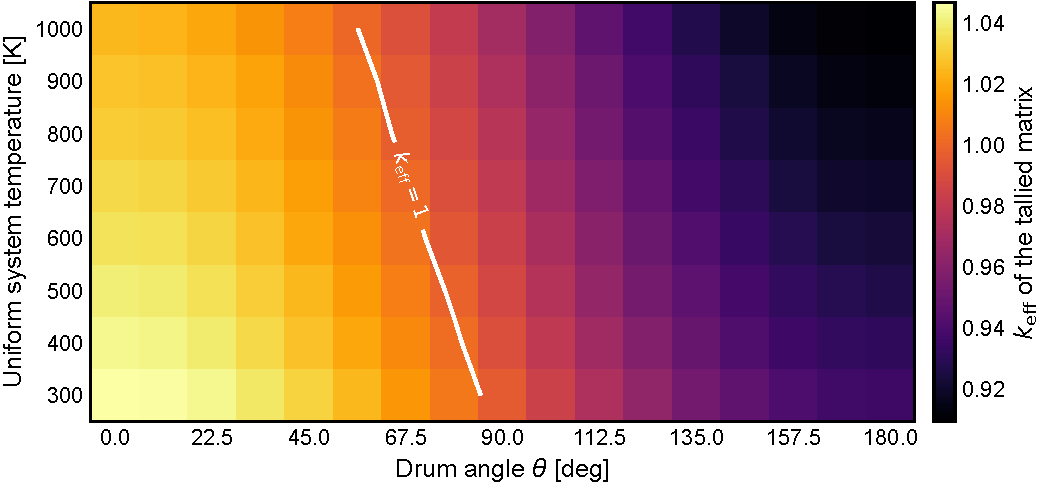
\includegraphics[width=\textwidth]{Chapter7/Figs/fmdb_keff_map.pdf}
  \caption[Multiplication factor of the tallied database]{Multiplication factor
  of the 136 tallied matrices of the database over the temperature and
  drum-angle grid, with the locus $k_{\mathrm{eff}}=1$.}
  \label{cs:fig:sanity}
\end{figure}

\subsection{Bilinear interpolation}\label{cs:sec:interp}

With two parameters, the coefficient-wise interpolation of
Sec.~\ref{fm:sec:database} is bilinear between the four entries that bracket
the target point. Let $d_T$ and $d_\theta$ be the indices of the database
levels immediately below the target temperature of cell $i$,
$\tilde T_{f,i}$, and the target angle $\tilde\theta$, so that
$\tilde T_{f,i}\in[T^{(d_T)},T^{(d_T+1)}]$ and
$\tilde\theta\in[\theta^{(d_\theta)},\theta^{(d_\theta+1)}]$. Then
%
\begin{equation}
  \tilde a_{ij}(\tilde T_{f,i},\tilde\theta) \;=\;
  \sum_{p=0}^{1}\sum_{q=0}^{1}
  w_T^{(p)}\!\left(\tilde T_{f,i}\right)\,
  w_\theta^{(q)}\!\left(\tilde\theta\right)\,
  a_{ij}^{(d_T+p,\;d_\theta+q)},
  \label{cs:eq:interp}
\end{equation}
%
where $a_{ij}^{(d_T+p,\,d_\theta+q)}$ is the coefficient tallied at the
corresponding grid point and the weights are the linear ones,
$w_T^{(1)} = (\tilde T_{f,i} - T^{(d_T)})/(T^{(d_T+1)} - T^{(d_T)})$,
$w_T^{(0)} = 1 - w_T^{(1)}$, and likewise for $\theta$. The temperature that
selects the position on the temperature axis is that of the destination cell
$i$, the row of the coefficient, as stated in Sec.~\ref{fm:sec:database}; the
angle is common to the whole matrix. The linear scheme is adopted as the simplest candidate; more elaborate
interpolants, and in particular schemes that would reduce the number of
entries required, are left to future work.

\subsection{Selection of the database}\label{cs:sec:selection}

The number of entries required to reach a given accuracy cannot be stated
beforehand. It is therefore settled by a nested procedure: a coarse database is built first, its
adequacy is judged by reproducing a fixed set of reference calculations, and
if the root-mean-square of $\Delta k_{\mathrm{eff}}$ over the set does not
fall within the statistical uncertainty of the references, entries are added.
The reference states are the same for every candidate and are taken at the
midpoints between neighbouring points of the finest grid, where the
interpolation error is largest: five temperatures, 350, 550, 650, 750 and
\SI{950}{K}, combined with three angles, \ang{5.625}, \ang{84.375} and
\ang{174.375}, fifteen cases in all. More elaborate adaptive strategies exist;
the nested one is adopted deliberately for its transparency.

Three databases are compared in Fig.~\tref{cs:fig:nested}. They share the eight
temperature levels and differ only in the drum axis: seventeen angles in steps
of \ang{11.25} for Database~1, nine in steps of \ang{22.5} for Database~2 and
five in steps of \ang{45} for Database~3, each database containing the coarser
ones. Only the drum axis is
refined because the rotation of the drums acts on the reactivity, and hence
on the coefficients, more strongly and less linearly than the temperature
does, as also observed on a research reactor with control rods
\cite{RauWaltersNSE2021}.

\begin{figure}[htbp]
  \centering
  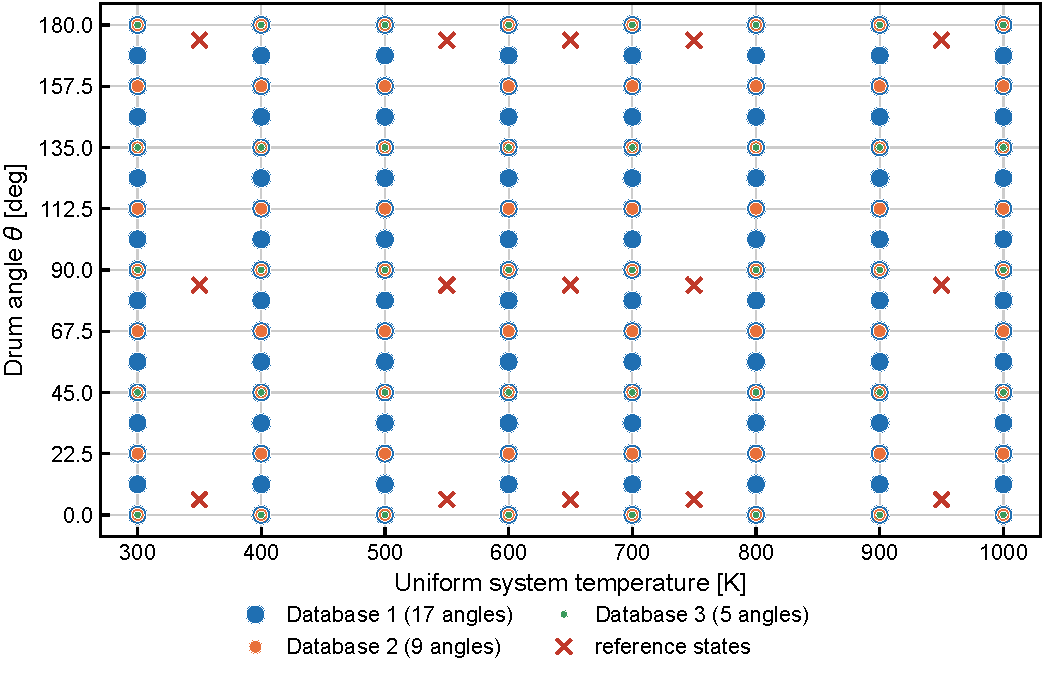
\includegraphics[width=\textwidth]{Chapter7/Figs/nested_databases.pdf}
  \caption[The three nested databases]{Grid points of the three nested
  databases over temperature and drum angle, and the fifteen reference states
  used to compare them (crosses). Database~1, the finest, contains the other
  two.}
  \label{cs:fig:nested}
\end{figure}

Figure~\tref{cs:fig:dbsel} shows $\Delta k_{\mathrm{eff}}$ between the
interpolated matrix and the reference calculation for the fifteen cases and
the three databases, and Table~\tref{cs:tab:dbsel} summarizes the metrics of
Sec.~\ref{fm:sec:metrics}. The root-mean-square deviation on the
multiplication factor falls from 165~pcm with Database~3 to 74~pcm with
Database~2 and to 29~pcm with Database~1, where most of the cases fall within
the statistical uncertainty of the references; the fission source improves
less, from \SI{1.1}{\percent} to \SI{0.8}{\percent}, since the source shape is
less sensitive to the angle than the eigenvalue is. Database~1 is adopted for the remainder of Part~II and is referred to simply
as ``the database'' hereafter.

\begin{figure}[htbp]
  \centering
  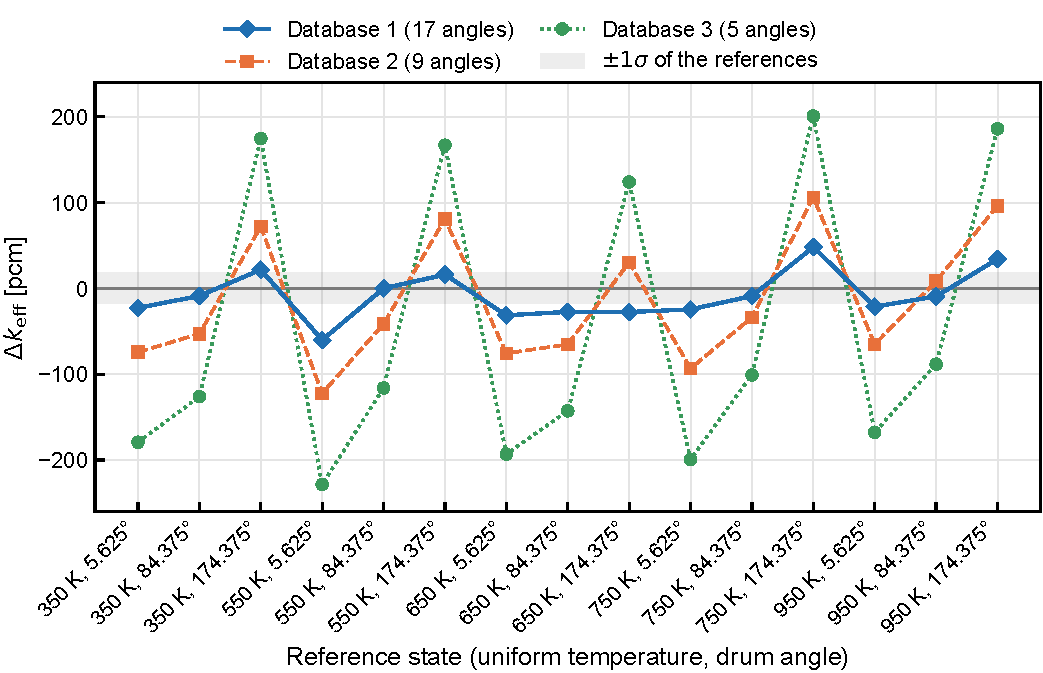
\includegraphics[width=\textwidth]{Chapter7/Figs/database_selection_dk.pdf}
  \caption[Interpolation error for the three databases]{Deviation of the
  multiplication factor of the interpolated matrix from the reference
  calculation at the fifteen reference states, for the three nested databases,
  with the $1\sigma$ statistical uncertainty of the references.}
  \label{cs:fig:dbsel}
\end{figure}

\begin{table}[htbp]
  \centering
  \caption[Interpolation error for the three databases]{Interpolation error
  over the fifteen reference states for the three nested databases: smallest,
  largest and root-mean-square absolute deviation of the multiplication factor,
  root-mean-square deviation of the fission source and largest local
  deviation.}
  \label{cs:tab:dbsel}
  \begin{tabular}{lccccc}
    \toprule
    & \multicolumn{3}{c}{$|\Delta k_{\mathrm{eff}}|$ (pcm)} &
    RMSE-$\tilde F$ (\%) & $\max|\delta\tilde F_i|$ (\%) \\
    \cmidrule(lr){2-4}
    & min & max & RMSE & & \\
    \midrule
    Database 1 (17 angles) &  0.1 &  61.0 &  28.5 & 0.82 & 1.2 \\
    Database 2 (9 angles)  &  8.4 & 122.8 &  74.2 & 1.10 & 1.6 \\
    Database 3 (5 angles)  & 87.9 & 228.7 & 164.9 & 1.12 & 2.4 \\
    \bottomrule
  \end{tabular}
\end{table}

\section{Power and fuel temperature correlation}\label{cs:sec:correlation}

No heat transfer calculation is performed in this work: neither a conduction model
of the assembly nor a model of the heat pipes is coupled to the fission
matrix. The fuel temperature field that enters the interpolation is obtained
from the reactor power and from the fission source through a prescribed
correlation, under two assumptions:
\begin{itemize}
  \item the average fuel temperature scales linearly with the power;
  \item the spatial distribution of the temperature is proportional to that of
  the fission source, $T_{f,i}\propto\tilde F_i$.
\end{itemize}
For cell $i$,
%
\begin{equation}
  T_{f,i} \;=\; \frac{P}{P_N}\,\xi_i + T_{\min,\mathrm{DB}},
  \qquad
  \xi_i \;=\; \frac{\tilde F_i - \min(\tilde{\mathbf F})}
                   {\max(\tilde{\mathbf F}) - \min(\tilde{\mathbf F})}\,
              \Delta T_{\mathrm{range}} + \big(T_{f,\min} - T_{\min,\mathrm{DB}}\big),
  \label{cs:eq:correlation}
\end{equation}
%
where $P$ is the reactor power, the independent variable, $P_N=\SI{2}{MW}$ its
nominal value, $T_{\min,\mathrm{DB}}=\SI{300}{K}$ the lowest temperature of
the database, and $T_{f,\min}$ and $\Delta T_{\mathrm{range}}$ are the minimum
fuel temperature and the temperature spread inside the core at nominal power,
which have to be provided as inputs. Throughout Part~II they are
$T_{f,\min}=\SI{823}{K}$ and $\Delta T_{\mathrm{range}}=\SI{51}{K}$. These values
are of the order of those of a high-fidelity simulation of the same core,
performed with the MOOSE framework \cite{giudicelli2024moose} at nominal power
with the drums fully extracted. Since the coldest cell of the core must not
exceed the highest temperature of the database, $T_{\max,\mathrm{DB}}=\SI{1000}{K}$,
the correlation is valid up to a maximum power
%
\begin{equation}
  P_{\max} \;=\; \frac{\big(T_{\max,\mathrm{DB}} - T_{\min,\mathrm{DB}}\big)\,P_N}
                      {\Delta T_{\mathrm{range}} + \big(T_{f,\min} - T_{\min,\mathrm{DB}}\big)},
  \label{cs:eq:pmax}
\end{equation}
%
which with the parameters above is \SI{2.44}{MW}. Powers beyond that limit
would require entries at higher uniform temperatures.

Three properties of this correlation determine what the verification of the
following sections can and cannot measure:
\begin{itemize}
  \item it is local and instantaneous: each cell is mapped on its own, with no
  conduction between cells and no dynamics of the heat pipes;
  \item it is normalized: the coldest and the hottest cell sit at the two ends of
  the interval by construction, so that what Eq.~(\ref{cs:eq:correlation})
  provides is the spatial redistribution of the temperature, which assemblies
  are hot and which are cold, and not the absolute spread, which is fixed
  \emph{a priori} at each power;
  \item it is shared by the workflow and by the reference calculations against
  which the workflow is verified: the references impose the same temperature
  profile through the multiphysics interface of Serpent.
\end{itemize}
The deviations reported in this chapter
therefore measure the accuracy of the fission matrix interpolation and of the
burnup correction, and not that of a heat transfer model. The coupling of the method
with a dedicated heat transfer model, and with a heat-pipe model in particular, is
left to future developments.

\section{The criticality search algorithm}\label{cs:sec:algorithm}

The power and fuel temperature correlation of Eq.~(\ref{cs:eq:correlation})
makes it possible to automate both the estimation of the fuel temperature
field and the search for the drum angle at which $k_{\mathrm{eff}}=1$. The
thermal feedback on the fission source is thereby taken into account only
approximately, since the temperature field is prescribed by the correlation
and not computed by a heat transfer model. The algorithm follows the scheme
proposed for a research reactor with control rods \cite{Topham2020} and
consists of two nested loops around the interpolated matrix. It is described
here for a fixed composition of the fuel; burnup enters further on, where the
same search is repeated at every time step of the cycle.

\begin{enumerate}
  \item \textbf{Initialization.} The drum angle is set to $\theta=\ang{0}$, the
  fission source to a flat guess, and the power $P$ and the parameters
  $T_{f,\min}$ and $\Delta T_{\mathrm{range}}$ of the correlation are assigned.
  \item \textbf{Neutronic--thermal equilibrium at fixed angle} (inner loop).
  \begin{enumerate}
    \item the fuel temperature field is estimated from the current fission
    source with Eq.~(\ref{cs:eq:correlation});
    \item the matrix is interpolated at that field and at the current angle
    with Eq.~(\ref{cs:eq:interp}), and the eigenproblem
    (\ref{fm:eq:eigen}) is solved for $\tilde k_{\mathrm{eff}}$ and
    $\tilde{\mathbf F}$;
    \item the temperature field is re-estimated from the new source;
    \item if the field differs from the previous one by more than
    $\epsilon=\SI{0.5}{\percent}$, the loop returns to step (b).
  \end{enumerate}
  \item \textbf{Criticality check} (outer loop). If
  $|\tilde k_{\mathrm{eff}}-1|<\delta$, where the tolerance $\delta$ is \SI{1}{pcm}
  when the uncertainty affecting the fission matrix is neglected, the state is
  critical; otherwise the
  angle is updated by bisection on $[\ang{0},\ang{180}]$, rotating the absorber
  towards the core when the system is supercritical and away from it when it
  is subcritical, and the algorithm returns to step 2.
  \item \textbf{Finalization.} The critical drum angle, the temperature field
  and the fission source of the converged state are stored.
\end{enumerate}

When the statistical uncertainty of the database is propagated, as described
in the next section, the search stops instead when the $\pm1\sigma$ band of the
last two iterates contains $k_{\mathrm{eff}}=1$: the drum angle is not resolved beyond the statistical
resolution of the database, and the condition on two consecutive iterates
avoids stopping on a single favourable bisection step.

In the cycle analysis the search is embedded in a further loop, which advances
the burnup of the fuel from one time step to the next and repeats the search at
every step on the fission matrix corrected for the fuel composition at that
time. A termination condition closes this loop: if the core is subcritical
with the drums fully extracted, criticality cannot be restored, and that
condition defines the end of the cycle life. Figure~\tref{cs:fig:flow-search}
draws the search at fixed composition; its extension to the cycle is drawn in
Fig.~\tref{cs:fig:flow}. Each outer iteration requires several evaluations of
the fission matrix, one per pass of the inner loop; a warm start on the
fission source of the previous iteration keeps the number of passes close to
one.

\begin{figure}[htbp]
  \centering
  \resizebox{\textwidth}{!}{%
  \begin{tikzpicture}[
    font=\small,
    node distance = 5mm and 13mm,
    base/.style  = {rectangle, rounded corners=1.5pt, align=center, inner sep=4.5pt,
                    minimum height=10mm, text width=68mm},
    old/.style   = {base, draw=black!55, line width=.5pt},
    round/.style = {rounded corners=4mm, fill=ga!55},
    serp/.style  = {old, fill=serpent!55, text width=38mm},
    fm/.style    = {old, fill=nnc!28},
    grey/.style  = {old, fill=black!8},
    dec/.style   = {diamond, aspect=2.3, draw=black!55, fill=ga!45, align=center,
                    inner sep=1pt, text width=38mm, font=\footnotesize},
    arO/.style   = {-{Latex[length=2mm]}, draw=black!65, line width=.55pt},
    lbl/.style   = {font=\footnotesize, inner sep=2pt},
  ]
  \node[grey] (start) {power $P$; parameters $T_{f,\min}$ and $\Delta T_{\mathrm{range}}$;\\
                       drum angle $\theta=\ang{0}$; initial guess of the fission source: flat};
  \node[old, below=of start] (temp) {fuel temperature field $T_{f,i}$ from
                       $\tilde{\mathbf F}$ and $P$, Eq.~(\ref{cs:eq:correlation})};
  \node[fm, below=of temp] (interp) {interpolated matrix
                       $\tilde a_{ij}(\tilde T_{f,i},\tilde\theta)$, Eq.~(\ref{cs:eq:interp})};
  \node[fm, below=of interp] (eig) {eigenproblem
                       $\tilde{\mathbf A}\,\tilde{\mathbf F}=\tilde k_{\mathrm{eff}}\,\tilde{\mathbf F}$};
  \node[dec, below=of eig] (dT) {temperature field changed\\by less than $\epsilon$?};
  \node[dec, below=of dT] (crit) {$|\tilde k_{\mathrm{eff}}-1|<\delta$?};
  \node[grey, below=of crit] (end) {critical state: critical drum angle
                       $\theta_{\mathrm{crit}}$,\\ temperature field $T_{f,i}$,
                       fission source $\tilde{\mathbf F}$};
  \node[serp, right=of interp] (db) {database of tallied matrices,
                       Sec.~\ref{cs:sec:database}};
  \node[old, round, right=of crit, text width=28mm] (bis) {bisection on $\theta$};
  \coordinate (rx) at ($(temp.east)+(70mm,0)$);

  \draw[arO] (start) -- (temp);
  \draw[arO] (temp) -- (interp);
  \draw[arO] (interp) -- (eig);
  \draw[arO] (eig) -- (dT);
  \draw[arO] (dT) -- node[lbl, right] {yes} (crit);
  \draw[arO] (crit) -- node[lbl, right] {yes} (end);
  \draw[arO] (db) -- (interp);
  \draw[arO] (dT.west) -- ++(-9mm,0) node[lbl, above, xshift=4mm] {no}
             |- (temp.west);
  \draw[arO] (crit) -- node[lbl, above] {no} (bis);
  \draw[arO] (bis.east) -- (bis.east -| rx) -- (rx |- temp.east) -- (temp.east);

  \begin{scope}[on background layer]
    \node[fill=ga!12, rounded corners=2.5mm, fit=(temp)(interp)(eig)(dT),
          inner sep=3.5mm] {};
  \end{scope}
  \end{tikzpicture}}
  \caption[The criticality search]{The criticality search. The shaded area
  encloses the inner loop, the neutronic--thermal equilibrium at fixed drum
  angle; the outer loop is the bisection on the drum angle. The tolerance
  $\delta$ is \SI{1}{pcm} when the uncertainty affecting the fission matrix is
  neglected; with the uncertainty ensemble the test on $\tilde k_{\mathrm{eff}}$
  is replaced by a statistical criterion. In the cycle analysis this search is
  repeated at every time step, on the matrix corrected for burnup, inside an
  outer loop that advances the burnup of each cell (Fig.~\ref{cs:fig:flow}).}
  \label{cs:fig:flow-search}
\end{figure}

\subsection{Uncertainty of the search results}\label{cs:sec:ensemble}

The uncertainty of the database is propagated with the ensemble method of
Sec.~\ref{fm:sec:uq}, in the following form. The uncertainty of the tallied
coefficients is systematic with respect to the search: the database is a
single set of tallies, shared by every evaluation the search performs, so that
its statistical error does not average out from one evaluation to the next. It
is therefore represented
by a fixed ensemble of database realizations. In realization $r$ every
coefficient is drawn from a Gaussian centred on its tallied value, with
standard deviation equal to its tallied uncertainty, independently of all the
others and truncated at zero; the realizations are generated once from a fixed
seed and kept in memory, so that realization $r$ is the same database wherever
it is used and all the results of the chapter are self-consistent. Only the
temperature levels that the search can reach at the given power are perturbed:
at fixed power, Eq.~(\ref{cs:eq:correlation}) confines the profile to a single
interval of the temperature grid, and the remaining coefficients are never
read.

At every state the search visits, the interpolated matrix is built from each
realization and the eigenproblem is solved; the standard deviation of the
eigenvalues over the ensemble is $\sigma_k$, while the estimate itself is
evaluated on the tallied database. The uncertainty of the converged drum angle
follows from a first-order expansion around the critical angle
$\theta_{\mathrm{crit}}$ found on the tallied database, where
$k_{\mathrm{eff}}(\theta_{\mathrm{crit}})=1$. A search run on realization $r$
converges instead at the angle $\theta^{(r)}$ at which the multiplication
factor of that realization, $k^{(r)}_{\mathrm{eff}}$, equals one. Linearizing
$k^{(r)}_{\mathrm{eff}}(\theta)$ around $\theta_{\mathrm{crit}}$, that is,
replacing the curve with its tangent, and neglecting the change of its slope
from one realization to another, gives
%
\begin{equation*}
  \theta^{(r)}-\theta_{\mathrm{crit}} \;\simeq\;
  -\,\frac{k^{(r)}_{\mathrm{eff}}(\theta_{\mathrm{crit}})-1}
          {\mathrm d k_{\mathrm{eff}}/\mathrm d\theta},
\end{equation*}
%
so that the error on the multiplication factor at fixed angle is converted
into an error on the angle through the local differential drum worth
$\mathrm d k_{\mathrm{eff}}/\mathrm d\theta$. The standard deviation of the
numerator over the ensemble is $\sigma_k$, and that of the angle is therefore
%
\begin{equation}
  \sigma_\theta \;=\; \frac{\sigma_k}{\,|\mathrm d k_{\mathrm{eff}}/\mathrm d\theta|\,},
  \label{cs:eq:sigmatheta}
\end{equation}
%
with the derivative evaluated by two additional eigenvalue solutions at
$\pm\ang{1}$ from the converged angle. Equation~(\ref{cs:eq:sigmatheta}) is an
approximation, since the multiplication factor is not a linear function of the
drum angle: the differential drum worth changes as the drums are withdrawn. It
holds as long as the curve departs little from its tangent over the width of
the uncertainty band, and it is verified against 50 complete searches per
state, one per database realization: the two estimates of $\sigma_\theta$
agree within \SI{3}{\percent}. The same
$\sigma_k$ drives the statistical stopping criterion of the search.

The size of the ensemble is chosen after checking the convergence of
$\sigma_k$. With twenty realizations $\sigma_k$ is underestimated by 10 to
\SI{15}{\percent} and varies by as much between independent groups of twenty;
with fifty it is within \SI{5}{\percent} of its value at two hundred. Fifty
realizations are used along the cycle, Sec.~\ref{cs:sec:cycle}, and one
hundred in the single search at nominal power of the next section. As
discussed in Sec.~\ref{fm:sec:uq}, perturbing the coefficients independently
neglects the correlations among the tallies of one run, so that the bands are
conservative: the replicate comparisons of Sec.~\ref{cs:sec:hypotheses}
indicate that they overestimate the observed scatter by roughly a factor 1.5.

\subsection{Convergence at nominal power}\label{cs:sec:convergence}

Figure~\tref{cs:fig:search} shows one search at $P=\SI{2}{MW}$ and fresh fuel,
iteration by iteration: the multiplication factor and the drum angle returned
by each outer iteration, with the cumulative computing time on the upper axis.
Each outer iteration comprises an inner loop and, once the iterates enter the
stopping region, the evaluation of the whole ensemble, so that the times on
the upper axis are the total cost of each step, uncertainty quantification
included. The search converges in 12 outer iterations and \SI{1.1}{s} on a single
core; the run comprises 16 nominal evaluations of the matrix and 7
sweeps of the 100 realizations. The critical angle is
$\theta_{\mathrm{crit}}=\ang{62.31}\pm\ang{0.14}$, the uncertainty being that
of Eq.~(\ref{cs:eq:sigmatheta}), and the multiplication factor at convergence
is $1.00004\pm11$~pcm.

\begin{figure}[htbp]
  \centering
  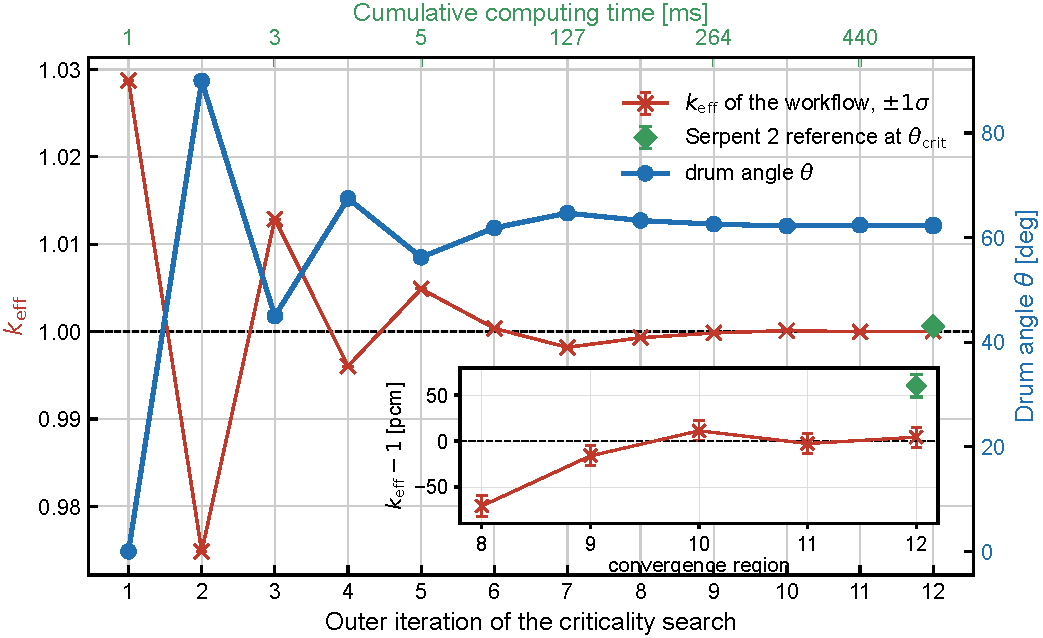
\includegraphics[width=\textwidth]{Chapter7/Figs/search_convergence.pdf}
  \caption[Convergence of the criticality search at nominal power]{Criticality
  search at nominal power and fresh fuel: multiplication factor (left axis) and
  drum angle (right axis) at each outer iteration, with the cumulative computing
  time on the upper axis, uncertainty quantification included. The inset
  resolves the convergence region in pcm, with the $\pm2\sigma$ bands of the
  ensemble and of the reference Serpent~2 calculation at the drum angle
  returned by the search.}
  \label{cs:fig:search}
\end{figure}

A reference Serpent~2 criticality calculation at the converged state, drums at
the angle returned by the search and the converged temperature field imposed
through the multiphysics interface, gives $k_{\mathrm{eff}}=1.00060\pm12$~pcm.
The deviation of the workflow from the reference is therefore $-56\pm16$~pcm,
where the uncertainty combines the two contributions of
Eq.~(\ref{fm:eq:sigma}). At $3.4$ standard deviations from zero, the deviation cannot be attributed to
statistical noise: it is the interpolation residual of the database at this
state, of the same magnitude as the residuals of Table~\tref{cs:tab:dbsel},
and it persists unchanged along the whole cycle
(Sec.~\ref{cs:sec:cycle-results}).

The cost of the search is dominated by the eigenvalue solutions (see
Fig.~\tref{cs:fig:searchcost}). When the Monte Carlo uncertainty of the
database is neglected, that is, with the \SI{1}{pcm} criterion and no
ensemble, a search converges in 13 outer iterations and 17 evaluations of the
matrix, one per pass of the inner loop, since four of the iterations require a
second pass. It takes \SI{29}{ms} on one core, the average of 20 repetitions of
the same search, since a single search is too short to be timed accurately;
\SI{77}{\percent}
of the time is the eigenvalue solution, \SI{17}{\percent} the interpolation
and \SI{6}{\percent} the inner loop with the correlation. With the ensemble, \SI{97}{\percent} of the \SI{1.1}{s} is spent in the
uncertainty quantification, which likewise consists mostly of eigenvalue
solutions. For comparison, one criticality calculation of
the database costs about \SI{63}{CPU\,h}, that is, about \SI{2.1}{h} on the
thirty-core workstation on which the database is generated, described further
on; a Monte Carlo search with the 12 outer iterations of the search with the
ensemble would require about one
day of wall-clock time on that machine, against one second for the present
workflow, and each additional Monte Carlo search would cost the same again,
whereas the cost of the database is incurred only once.

The same comparison explains why, when the neutronic model is Monte Carlo, the
design of the search algorithm becomes a research problem in its own right. Each evaluation of
$k_{\mathrm{eff}}$ then costs tens of CPU hours, so that the number of
iterations decides the cost of the search, and it returns an estimate with a
statistical uncertainty that can disrupt the progression of a root-finding
scheme. \citet{PriceRoskoffPNE2023} developed for this purpose secant-type
methods with explicit provisions for the statistical uncertainty of the
estimates, applied to the drum position of micro reactors, and the same
method was later embedded in a multiphysics depletion workflow that searches
the critical drum position at every burnup point \cite{PriceNSE2024}. With
the fission matrix each evaluation involves no new Monte Carlo sampling and
costs milliseconds, and the plain bisection described above is sufficient.

\begin{figure}[htbp]
  \centering
  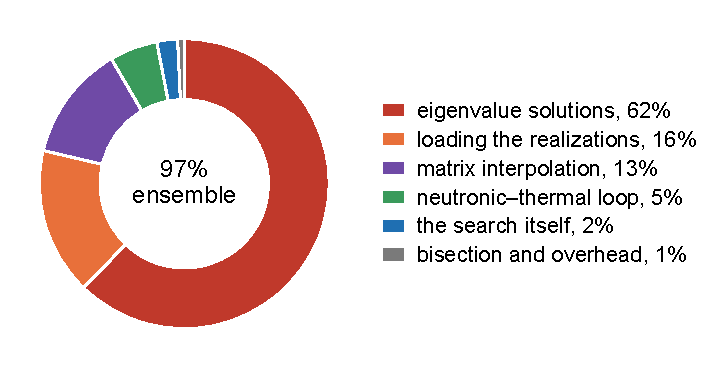
\includegraphics[width=0.75\textwidth]{Chapter7/Figs/search_cost.pdf}
  \caption[Composition of the cost of one search]{Composition of the computing
  time of one search with the ensemble, measured on an instrumented run with
  the steps timed one by one. The uncertainty quantification, that is,
  everything but the search itself and the bisection, takes
  \SI{97}{\percent} of the total, and most of it is the eigenvalue solution of
  the realizations.}
  \label{cs:fig:searchcost}
\end{figure}

\subsection{Critical drum angle against power at beginning of life}\label{cs:sec:bol}

Figure~\tref{cs:fig:power} shows the critical drum angle as a function of the
power, from zero to \SI{2.4}{MW}, obtained with the \SI{1}{pcm} criterion,
which neglects the Monte Carlo uncertainty of the database,
together with the minimum and maximum fuel temperature of the core at each
power. The relation is close to linear: the critical angle moves from
\ang{84.8} at zero power to \ang{62.4} at nominal power and to about \ang{58}
at \SI{2.4}{MW}; the curvature is due to the thermal feedback, which is small
compared with the drum worth. At nominal power the search gives
$\theta_{\mathrm{crit}}=\ang{62.36}$ with a temperature range of
\SIrange{823}{874}{K}, fixed by construction of the correlation. The zero-power point is a check that involves
no temperature interpolation: at $P=0$ the system is uniform at \SI{300}{K},
one of the database levels, and the critical angle of \ang{84.81} returned by
the search compares with \ang{84.90} read directly from the crossing of unity
of the tallied $k_{\mathrm{eff}}(\theta)$ at that temperature.

\begin{figure}[htbp]
  \centering
  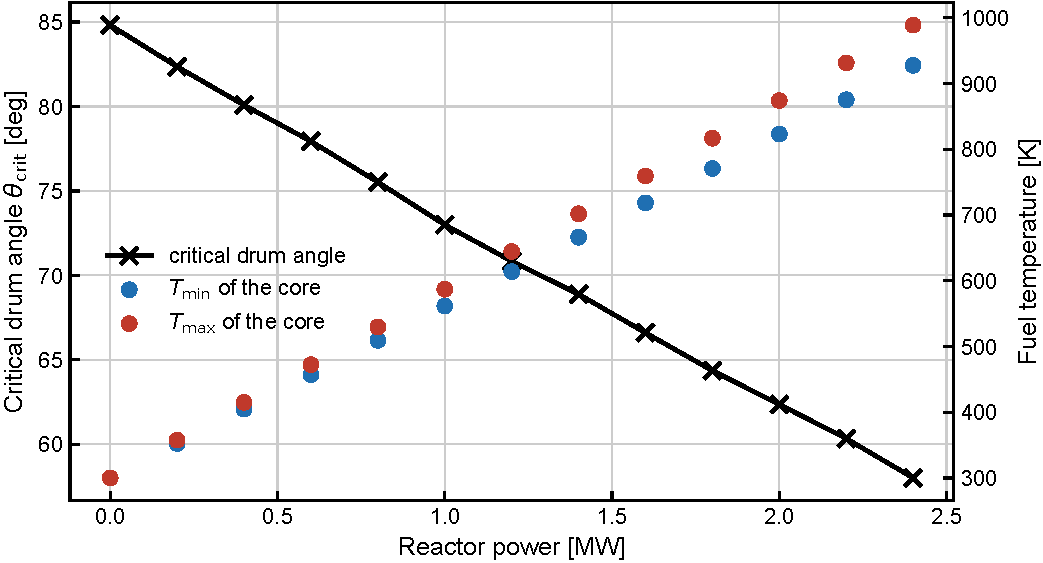
\includegraphics[width=\textwidth]{Chapter7/Figs/bol_angle_vs_power.pdf}
  \caption[Critical drum angle against power]{Critical drum angle at beginning
  of life as a function of the reactor power, from zero to \SI{2.4}{MW}
  (crosses, left axis), with the minimum and maximum fuel temperature of the
  core at each power (right axis).}
  \label{cs:fig:power}
\end{figure}

The verification of the search against reference calculations at powers other
than the nominal one was carried out, in the original study, with the
Reflector Correction Ratio applied to the interpolated matrix. Those results depend on the reflector correction, which is the subject of
Chapter~\ref{ch:correction-ratios}, and are not reported; the verification of
the uncorrected workflow rests on the nominal-power case above and on the
twelve reference states of the cycle analysis of
Sec.~\ref{cs:sec:cycle-results}, all at nominal power. The
construction does not depend on the power level, since the temperature axis of
the database carries it, and the same procedure applies at any power below
$P_{\max}$.

\section{Extension to burnup}\label{cs:sec:burnup}

\subsection{The size of the database}

Fuel depletion changes the coefficients of the fission matrix through the
composition of the fuel, and a cycle analysis needs those changes: the drum
angle that keeps the core critical, the remaining excess reactivity and the
cycle length. Burnup-dependent fission-matrix methods exist, for instance the
burnup algorithm of the RAPID code system \cite{pungercic2023brapid} and the
coupling of the fission matrix with depletion of \citet{he2024combined}.
The challenge addressed here is different: the aim is to add burnup to a
database that already spans temperature and drum angle while minimizing its
size.

The direct extension is a third dimension, one matrix for every combination of
temperature level, drum angle and burnup step. With the 12 burnup steps used below, this amounts to
$8\times17\times12=1632$ criticality calculations, i.e., 12 times the existing
campaign, each requiring the composition of its step and therefore a preceding
depletion calculation. The database would be multiplied by the number of
levels of every dimension added, the growth known as the curse of
dimensionality \cite{Bellman1957}, and the method would lose the separation on which
its economy rests, between a tallying campaign performed once and searches
that require no further transport calculation.

\subsection{The Burnup Correction Ratio}\label{cs:sec:bcr}

The composition effect is therefore factorized out of the interpolated matrix
through a correction ratio: a multiplicative factor applied element by
element to the interpolated matrix, built as the ratio of two matrices
tallied at reference conditions that differ in the effect of interest alone,
here the fuel composition. The interpolated coefficient is multiplied by a Burnup Correction Ratio (BCR), the ratio between the
coefficient tallied at a burnup snapshot and the coefficient tallied at the
fresh state, under fixed reference conditions:
%
\begin{equation}
  \tilde a^{*}_{ij}(\tilde T_{f,i},\tilde\theta,t) \;=\;
  \tilde a_{ij}(\tilde T_{f,i},\tilde\theta)\cdot \mathrm{BCR}_{ij}(t),
  \qquad
  \mathrm{BCR}_{ij}(t_s) \;=\; \frac{a^{\mathrm{snap}}_{ij}(t_s)}{a^{\mathrm{snap}}_{ij}(0)} .
  \label{cs:eq:bcr}
\end{equation}
%
Numerator and denominator are fission-matrix tallies at the same reference
conditions, drums fully extracted, $\theta_{\mathrm{ref}}=\ang{0}$, and the
nominal-power temperature state of the searches at beginning of life; they
differ only in the fuel composition, taken from a depletion history at the
snapshot times $t_s$. Between snapshots, the ratio is interpolated linearly in
time. Systematic effects common to numerator and denominator cancel in the
ratio, while the interpolated matrix keeps the temperature and drum
dependence.

Where the tallies resolve it, the burnup change of a coefficient is small, and
a ratio far from unity has no physical cause: it comes from a coefficient
tallied with few counts, in the numerator or in the denominator, since the
ratio of two such noisy estimates can exceed 2 or fall below 0.5, and a
coefficient that receives no score at the snapshot has a ratio of zero. The
ratio is therefore limited to the interval $[0.5,2]$: a ratio below 0.5 is set
to 0.5 and a ratio above 2 is set to 2, while a coefficient that receives no
score at the fresh state keeps a ratio of one. How many coefficients the limit
affects, and with what effect on the multiplication factor, is quantified
below, once the snapshot times have been introduced.

Equation~(\ref{cs:eq:bcr}) rests on three assumptions, each of which is
measured on a dedicated campaign later in the chapter:
\begin{itemize}
  \item \textbf{Angle independence.} The burnup response of a coefficient does
  not depend on the drum angle at which it is tallied.
  \item \textbf{Fixed temperature.} The burnup response of a coefficient does
  not depend on the temperature state.
  \item \textbf{Single history.} The compositions of one depletion history, run
  with the drums fully extracted, represent those of the operating reactor,
  whose drums follow the critical trajectory.
\end{itemize}

\subsection{The snapshot database}\label{cs:sec:snapshots}

The snapshot times are $t_s\in\{0,\,0.25,\,0.5,\,1,\,2,\,4,\,8,\,15,\,24,\,36,\,51,\,66\}$
months at nominal power. The grid is dense in the first two months and sparse
afterwards. Early in life, the fission-product inventory is furthest from
linear: the snapshots carry the build-up of $^{135}$Xe, which saturates within
days, and of $^{149}$Sm, which takes about two years at the low flux of this
VTB design, as the fuel inventory presented further on shows. Afterwards, the
evolution is close to linear, because the design has no burnable poisons. The
grid runs to 66 months, the end of the window analysed in this chapter, so
that the whole window is supported by the database and not by extrapolation;
the end of life, near month 70 as shown further on, lies just beyond it.

On this grid the limit of the ratio can be quantified. At 66 months, the
coefficients tallied with a relative uncertainty below \SI{2}{\percent} in both
numerator and denominator, which carry \SI{90}{\percent} of the weight of the
matrix, have ratios between 0.91 and 1.05. The limit acts on about
\SI{10}{\percent} of the coefficients at every snapshot time, from a quarter of
a month to 66 months, and therefore does not grow with burnup; those
coefficients carry \SI{0.02}{\percent} of the weight of the matrix, and at 66
months their treatment changes $k_{\mathrm{eff}}$ by \SI{5}{pcm}.

The campaign is split in two parts. One low-statistics depletion calculation,
$2\times10^{4}$ neutrons per cycle and 260 active cycles, at the reference
state gives the compositions at the snapshot times and writes a Serpent~2
restart file.
Twelve independent full-statistics transport calculations, with the same
population as the database entries and their own random-number seeds, read one
snapshot composition each from that file and tally the matrix. Numerator and
denominator of every ratio are therefore statistically independent runs. The
snapshot matrices have the same median relative uncertainty as the database,
\SI{9.2}{\percent}. The restart file makes every additional variant a
transport-only cost: the angle-resolved snapshots and the evolved-temperature
snapshot used to test the assumptions come from the same depletion. The
snapshot database receives the same ensemble treatment as the main database:
numerator and denominator of the ratio are perturbed independently, and every
uncertainty band of the cycle carries both databases.

Burnup has previously been introduced into fission matrix methods in two
forms. In the RAPID
code system the matrix is precomputed from fixed-source calculations at a
set of points in power and irradiation time and interpolated between them at
every depletion step \cite{pungercic2023brapid}; in the combined fission
matrix of \citet{he2024combined} the database matrices are corrected for the
evolution of the composition inside a transport--depletion loop. The
databases interpolated over temperature and control-rod position
\cite{Topham2020,RauWaltersNSE2021} do not include burnup, and the
multiplicative correction ratios of RAPID \cite{HeANE2019,HePNE2020} address
reflectors, heterogeneous assemblies and control rods. The scheme adopted
here differs from those in two respects. The snapshot matrices are tallied
whole-core, during criticality calculations restarted from a single
depletion run once at reference conditions, so that the compositions are
computed once and every matrix is a transport-only cost; and the ratio
between the burned and the fresh matrix scales, coefficient by coefficient, a
matrix interpolated over temperature and drum angle, so that burnup adds a
factor to the database and not another dimension.

\subsection{The quasi-static cycle}\label{cs:sec:cycle}

The workflow marches the cycle on an evolution grid, with sub-monthly steps in
the first two months and monthly steps afterwards, with 71 steps in total. At
every step the full criticality search described above runs on the corrected
matrix
of Eq.~(\ref{cs:eq:bcr}), so that drum position, temperature field and
fission source are updated together, consistently, at every step. The
cell-wise burnup advances with a predictor--corrector step,
%
\begin{equation}
  BU_i \;\leftarrow\; BU_i + \frac{P\,\bar F_i\,\Delta t}{m_i},
  \label{cs:eq:bustep}
\end{equation}
%
where $\bar F_i$ is the fission-source fraction of cell $i$ averaged over the
step and $m_i$ the heavy-metal mass of the cell, the total inventory of
\SI{448.5}{kg} being read from the Serpent output. The march ends when the
search can no longer restore criticality with the drums fully extracted.
Figure~\tref{cs:fig:flow} draws the complete scheme.

\begin{figure}[htbp]
  \centering
  \resizebox{\textwidth}{!}{%
  \begin{tikzpicture}[
    font=\small,
    node distance = 5mm and 13mm,
    base/.style  = {rectangle, rounded corners=1.5pt, align=center, inner sep=4.5pt,
                    minimum height=10mm, text width=68mm},
    old/.style   = {base, draw=black!55, line width=.5pt},
    new/.style   = {base, draw=newc, line width=1.3pt},
    round/.style = {rounded corners=4mm, fill=ga!55},
    serp/.style  = {old, fill=serpent!55, text width=38mm},
    serpN/.style = {new, fill=serpent!55, text width=38mm},
    fm/.style    = {old, fill=nnc!28},
    fmN/.style   = {new, fill=nnc!28},
    grey/.style  = {old, fill=black!8},
    greyN/.style = {new, fill=black!8},
    dec/.style   = {diamond, aspect=2.3, draw=black!55, fill=ga!45, align=center,
                    inner sep=1pt, text width=38mm, font=\footnotesize},
    decN/.style  = {dec, draw=newc, line width=1.3pt},
    arO/.style   = {-{Latex[length=2mm]}, draw=black!65, line width=.55pt},
    arN/.style   = {-{Latex[length=2mm]}, draw=newc, line width=1.1pt},
    lbl/.style   = {font=\footnotesize, inner sep=2pt},
  ]
  \node[greyN] (start) {time $t=0$, burnup $BU_i=0$; power $P$;\\
                       drum angle $\theta=\ang{0}$; flat fission source};
  \node[old, below=of start] (temp) {fuel temperature field $T_{f,i}$ from
                       $\tilde{\mathbf F}$ and $P$, Eq.~(\ref{cs:eq:correlation})};
  \node[fmN, below=of temp] (interp) {corrected matrix
                       $\tilde a^{*}_{ij}=\tilde a_{ij}(\tilde T_{f,i},\tilde\theta)\cdot\mathrm{BCR}_{ij}(t)$,
                       Eq.~(\ref{cs:eq:bcr})};
  \node[fm, below=of interp] (eig) {eigenproblem
                       $\tilde{\mathbf A}^{*}\tilde{\mathbf F}=\tilde k_{\mathrm{eff}}\,\tilde{\mathbf F}$};
  \node[dec, below=of eig] (dT) {temperature field changed\\by less than $\epsilon$?};
  \node[decN, below=of dT] (crit) {$\pm\sigma_k$ band of two iterates\\contains 1?};
  \node[greyN, below=of crit] (rec) {record $\theta_{\mathrm{crit}}(t)$ and $\sigma_\theta$,
                       Eq.~(\ref{cs:eq:sigmatheta});\\ advance the burnup $BU_i$, Eq.~(\ref{cs:eq:bustep})};
  \node[decN, below=of rec] (eol) {critical with the drums\\fully extracted?};
  \node[greyN, below=of eol] (end) {end of cycle life};
  \node[serp, right=of start] (db) {database of tallied matrices,
                       Sec.~\ref{cs:sec:database}};
  \node[serpN, right=of eig] (snap) {snapshot database,
                       $\mathrm{BCR}_{ij}(t)$, Sec.~\ref{cs:sec:snapshots}};
  \node[old, round, right=of crit, text width=28mm] (bis) {bisection on $\theta$};
  \coordinate (rx) at ($(temp.east)+(70mm,0)$);

  \draw[arN] (start) -- (temp);
  \draw[arO] (temp) -- (interp);
  \draw[arO] (interp) -- (eig);
  \draw[arO] (eig) -- (dT);
  \draw[arO] (dT) -- node[lbl, right] {yes} (crit);
  \draw[arN] (crit) -- node[lbl, right] {yes} (rec);
  \draw[arN] (rec) -- (eol);
  \draw[arN] (eol) -- node[lbl, right] {no} (end);
  \draw[arO] (db.west) -- ++(-4mm,0) |- ([yshift=3mm]interp.east);
  \draw[arN] (snap.west) -- ++(-4mm,0) |- ([yshift=-3mm]interp.east);
  \draw[arO] (dT.west) -- ++(-9mm,0) node[lbl, above, xshift=4mm] {no}
             |- (temp.west);
  \draw[arO] (crit) -- node[lbl, above] {no} (bis);
  \draw[arO] (bis.east) -- (bis.east -| rx) -- (rx |- temp.east) -- (temp.east);
  \draw[arN] (eol.west) -- ++(-16mm,0) node[lbl, above, xshift=8mm] {yes}
             |- node[lbl, left, pos=0.25] {$t\leftarrow t+\Delta t$} (start.west);

  \begin{scope}[on background layer]
    \node[fill=ga!12, rounded corners=2.5mm, fit=(temp)(interp)(eig)(dT),
          inner sep=3.5mm] {};
  \end{scope}

  \node[new, fill=white, below left=8mm and -44mm of end, text width=4mm,
        minimum height=4mm, inner sep=0pt] (lg1) {};
  \node[lbl, right=2mm of lg1, anchor=west] {introduced by the burnup extension};
  \node[old, fill=white, below=3mm of lg1, text width=4mm,
        minimum height=4mm, inner sep=0pt] (lg2) {};
  \node[lbl, right=2mm of lg2, anchor=west] {inherited from the search of Fig.~\tref{cs:fig:flow-search}};
  \end{tikzpicture}}
  \caption[The quasi-static cycle]{The quasi-static cycle. Boxes and arrows
  outlined in blue are introduced by the burnup extension, those with a thin
  grey outline are the search of Fig.~\ref{cs:fig:flow-search}. The shaded
  area encloses the inner loop; the outer loop is the bisection on the drum
  angle, stopped when, on two consecutive iterates, the $\pm\sigma_k$ band of
  the ensemble contains $k_{\mathrm{eff}}=1$; the outermost loop advances
  the cell-wise burnup and enters the next time step. Burnup enters only
  through the factor $\mathrm{BCR}_{ij}(t)$ of the corrected matrix.}
  \label{cs:fig:flow}
\end{figure}

\section{Results over the cycle}\label{cs:sec:cycle-results}

\subsection{The critical drum angle and its verification}

Figure~\tref{cs:fig:cycle} shows the critical drum angle over the 66-month
cycle at \SI{2}{MW}, up to a core-average burnup of \SI{8.96}{MWd/kg}, with
the $\pm1\sigma$ band of the fifty database realizations, and marks the
twelve states at which the workflow is verified. Each of them is an
independent Serpent~2 criticality calculation set up for the purpose, which
imposes the composition of that snapshot, the drums at the critical angle
returned by the workflow and the fuel temperature field of the converged
state. That field is computed by the workflow from the reactor power and the
fission source with the correlation of Eq.~(\ref{cs:eq:correlation}), and it
is imposed through the multiphysics interface, as in the reference calculation
at nominal power and fresh fuel described earlier. The drums move
monotonically from \ang{62.3} to \ang{12.0}. The build-up of $^{135}$Xe is
visible in the first week, where the angle drops from \ang{62.4} to
\ang{59.9}; the inset compares the quasi-static march with searches run
directly at the snapshot times, which coincide within the band.
Figure~\tref{cs:fig:cyclemaps} shows the normalized fission source of the
workflow at the twelve snapshot times, assembly-wise and axially integrated,
and its assembly-wise deviation from the reference calculations.

\begin{figure}[htbp]
  \centering
  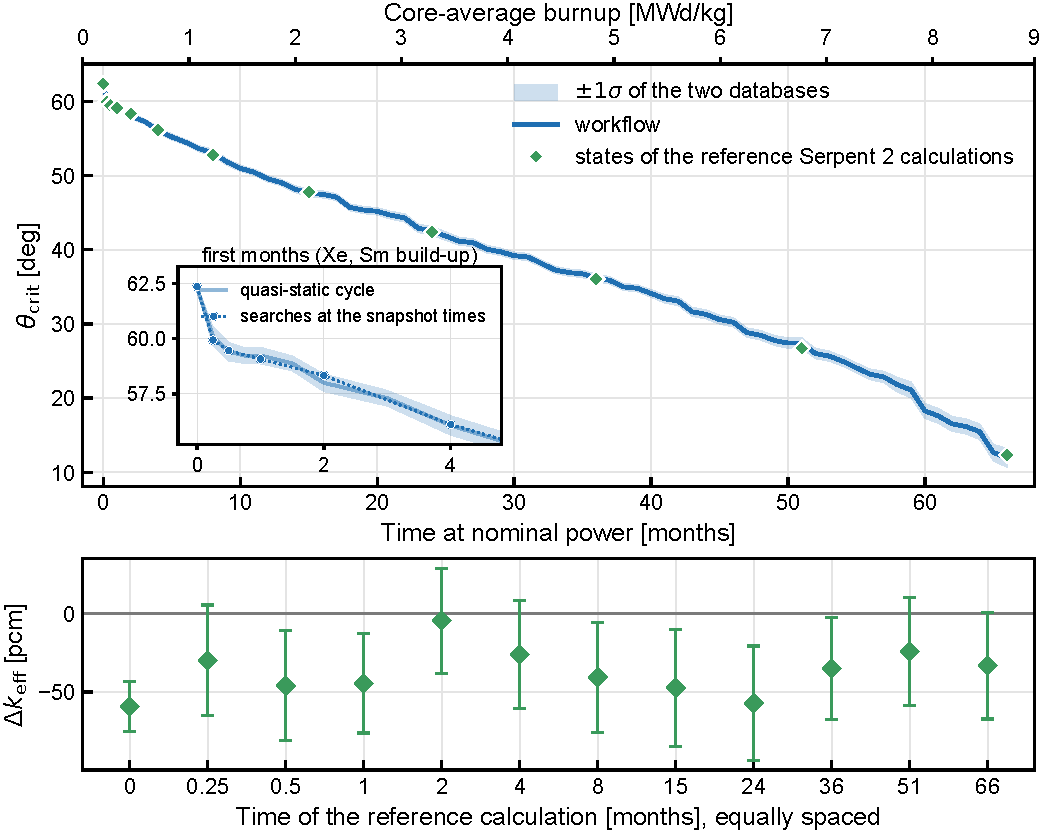
\includegraphics[width=\textwidth]{Chapter7/Figs/cycle_angle_verification.pdf}
  \caption[Critical drum angle over the cycle]{Upper panel: critical drum
  angle over the cycle at nominal power (core-average burnup on the upper
  axis), with the $\pm1\sigma$ band of the fifty database realizations and,
  in green, the twelve states at which independent reference Serpent~2
  calculations are run; the inset
  resolves the first months, where the isotopic settling takes place, and
  compares the quasi-static cycle with searches run directly at the snapshot
  times. Lower panel: deviation of the workflow multiplication factor from the
  reference at the twelve states, with the combined $\pm1\sigma$ uncertainty;
  the cases are equally spaced for readability.}
  \label{cs:fig:cycle}
\end{figure}

\begin{figure}[htbp]
  \centering
  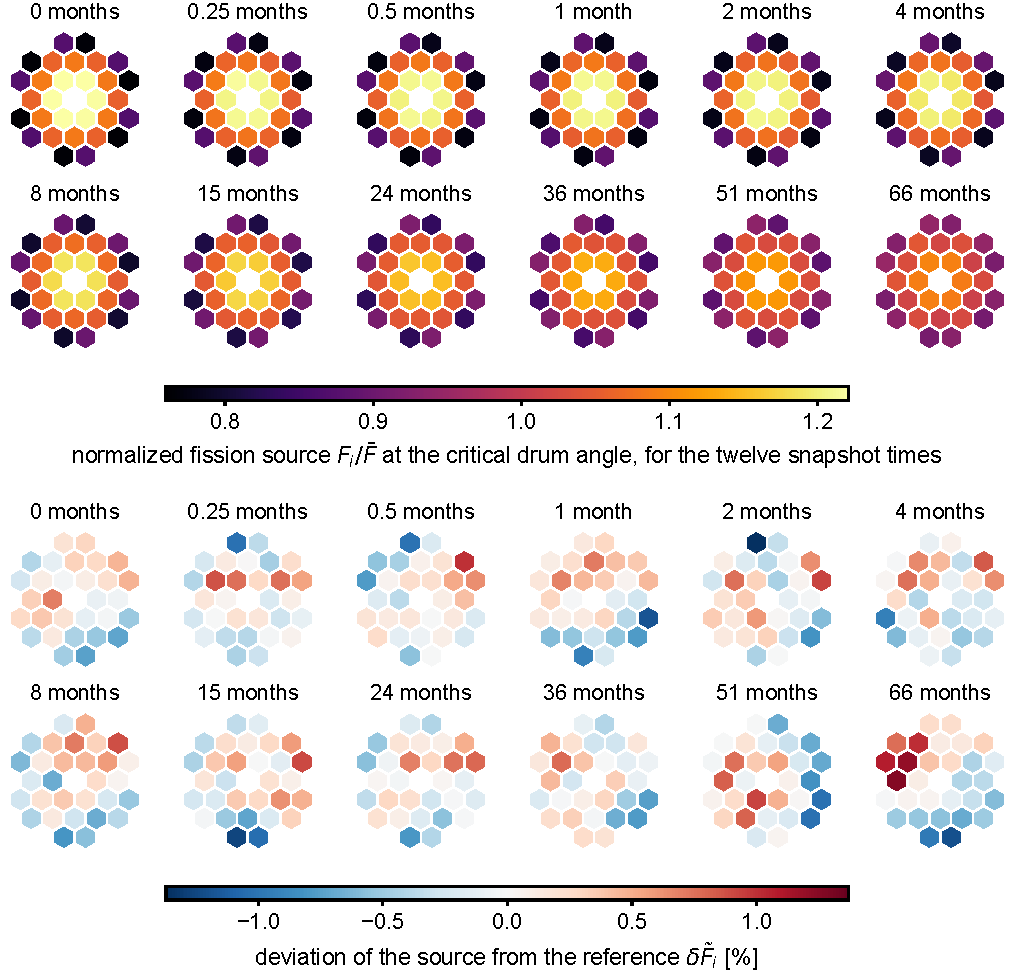
\includegraphics[width=\textwidth]{Chapter7/Figs/cycle_maps_critical.pdf}
  \caption[Fission source and its deviation over the cycle]{Assembly-wise,
  axially integrated fission source of the workflow at the critical drum angle
  of each of the twelve snapshot times (upper maps), and its deviation from
  the reference Serpent~2 calculation at the same state (lower maps).}
  \label{cs:fig:cyclemaps}
\end{figure}

Table~\tref{cs:tab:verification} lists the twelve comparisons between the
workflow and the reference calculations, the workflow being evaluated at
exactly the state imposed on each reference. The deviation
$\Delta k_{\mathrm{eff}}$ lies between $-59$ and $-5$~pcm over the whole cycle,
with a root-mean-square of \SI{40}{pcm}, against a combined statistical
uncertainty of 31 to \SI{37}{pcm}. The bias is already present at beginning of
life, where the correction ratio is identically one, and does not drift as
burnup proceeds: after beginning of life, the eleven points oscillate about
$-35$~pcm within their bands. The burnup correction therefore adds no
measurable error up to the burnup reached here. The assembly-wise fission source agrees with the
references to \SI{0.35}{\percent} on average and \SI{1.37}{\percent} at most.

\begin{table}[htbp]
  \centering
  \caption[Verification of the cycle against reference calculations]{Verification
  of the workflow at the twelve snapshot times: critical drum angle returned by
  the algorithm, multiplication factor of the reference Serpent~2 calculation at
  that state, deviation of the workflow from the reference and combined
  $1\sigma$ uncertainty.}
  \label{cs:tab:verification}
  \begin{tabular}{S[table-format=2.2] S[table-format=2.2] S[table-format=1.5] S[table-format=-2.0] S[table-format=2.0]}
    \toprule
    {$t$ (months)} & {$\theta_{\mathrm{crit}}$ (deg)} & {$k^{\mathrm{MC}}_{\mathrm{eff}}$} &
    {$\Delta k_{\mathrm{eff}}$ (pcm)} & {$\sigma_{\mathrm{tot}}$ (pcm)} \\
    \midrule
     0    & 62.36 & 1.00060 & -59 & 16 \\
     0.25 & 59.94 & 1.00030 & -30 & 35 \\
     0.5  & 59.46 & 1.00047 & -46 & 35 \\
     1    & 59.08 & 1.00045 & -44 & 31 \\
     2    & 58.34 & 1.00005 &  -5 & 33 \\
     4    & 56.12 & 1.00027 & -26 & 35 \\
     8    & 52.73 & 1.00041 & -41 & 35 \\
    15    & 47.77 & 1.00047 & -47 & 37 \\
    24    & 42.41 & 1.00058 & -57 & 36 \\
    36    & 36.06 & 1.00035 & -35 & 32 \\
    51    & 26.72 & 1.00025 & -24 & 34 \\
    66    & 12.35 & 1.00033 & -33 & 34 \\
    \bottomrule
  \end{tabular}
\end{table}

The two uncertainties of the results, on the eigenvalue and on the drum angle,
evolve differently along the cycle. The uncertainty on the eigenvalue, $\sigma_k$, grows from
\SI{11}{pcm} at beginning of life, where only the main database contributes,
to 30 to \SI{36}{pcm} once the snapshot tallies enter the ratio, and stays
nearly constant afterwards. The uncertainty on the angle, $\sigma_\theta$,
grows instead from \ang{0.14} to \ang{1.3}, because the differential drum
worth falls from 78 to \SI{25}{pcm} per degree as the drums are withdrawn:
the same uncertainty on $k_{\mathrm{eff}}$ maps onto a wider interval in
angle, and the band of Fig.~\tref{cs:fig:cycle} widens accordingly towards
the end of the cycle.

\subsection{Excess reactivity and cycle length}

The multiplication factor with the drums fully extracted, evaluated along the
cycle, sets the fuel cycle length when $k_{\mathrm{eff}}=1$ (see
Fig.~\tref{cs:fig:drumsout}). The excess reactivity starts at \SI{2870}{pcm}
at beginning of life. This value is read from the tallied database and is not
a free parameter. The reactivity decreases by \SI{500}{pcm} per year over the second
year and by \SI{376}{pcm} per year at the end of the window, that is, 307 and
\SI{231}{pcm} per \si{MWd/kg}; \SI{120}{pcm} are left at 66 months, so that
the end of life falls near month 70. The reference points of the figure are
the snapshot transports themselves, full-statistics calculations at
$\theta=\ang{0}$ with the composition of each snapshot, with their own
statistics. They are tallied at the reference temperature state, while the
workflow curve carries the evolved profile, a difference bounded by the
fixed-temperature test described further on. The combined
uncertainty of the two databases on the drums-out multiplication factor is 17
to \SI{36}{pcm}, and the assembly-wise error of the workflow source against
the references (see Fig.~\tref{cs:fig:drumsoutmaps}) is \SI{0.24}{\percent} on
average and \SI{0.79}{\percent} at most.

\begin{figure}[htbp]
  \centering
  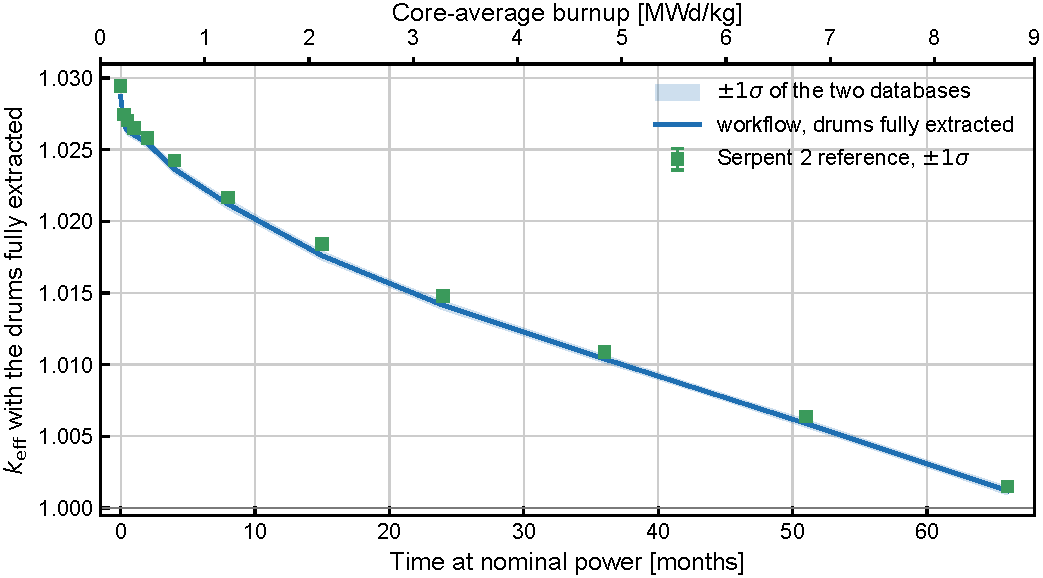
\includegraphics[width=\textwidth]{Chapter7/Figs/drums_out_reactivity.pdf}
  \caption[Excess reactivity over the cycle]{Multiplication factor with the
  drums fully extracted over the cycle: workflow with its $\pm1\sigma$ band and
  the twelve reference Serpent~2 calculations.}
  \label{cs:fig:drumsout}
\end{figure}

\begin{figure}[htbp]
  \centering
  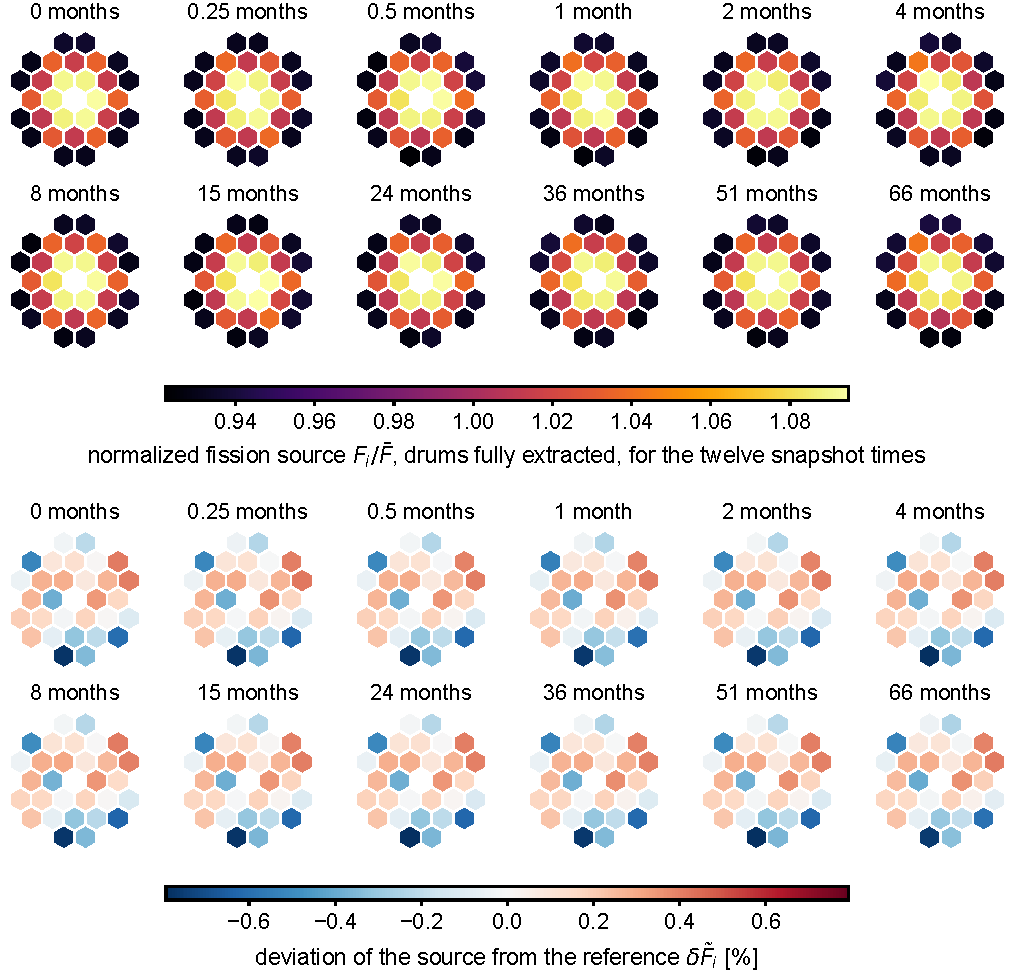
\includegraphics[width=\textwidth]{Chapter7/Figs/cycle_maps_drums_out.pdf}
  \caption[Fission source with the drums extracted]{Assembly-wise fission
  source of the workflow with the drums fully extracted at the twelve snapshot
  times (upper maps) and its deviation from the reference (lower maps); the
  maps of Fig.~\ref{cs:fig:cyclemaps} are instead at the critical drum position
  of each time.}
  \label{cs:fig:drumsoutmaps}
\end{figure}

\subsection{Fission source, temperature and fuel inventory}\label{cs:sec:inventory}

Without burnable poisons the cells with the highest source burn fastest and
lose local reactivity, so that the distribution flattens over the cycle, the
source decreasing in the central assemblies and increasing in the
drum-adjacent periphery. Figure~\tref{cs:fig:flattening}
shows the assembly peaking factor, which decreases from 1.221 to 1.096, and
the fuel temperature of the assemblies that are hottest and coldest at
beginning of life, which converge as the source flattens. The flattening is
favourable to the operation of the core: as the fuel is burnt, the power of
the most loaded assembly approaches the core average. The maps of
Fig.~\tref{cs:fig:bolmaps} locate the change: the source of the central
assemblies decreases by \SI{11}{\percent} and that of the periphery increases
by \SI{21}{\percent} between beginning and end of the window, and the
temperature field of Eq.~(\ref{cs:eq:correlation}) follows, with
assembly-wise changes between $-2.7$ and $+5.2$~K. With that correlation the global extremes of
the temperature are fixed at each power by construction; the physical content
of the maps is the spatial redistribution.

\begin{figure}[htbp]
  \centering
  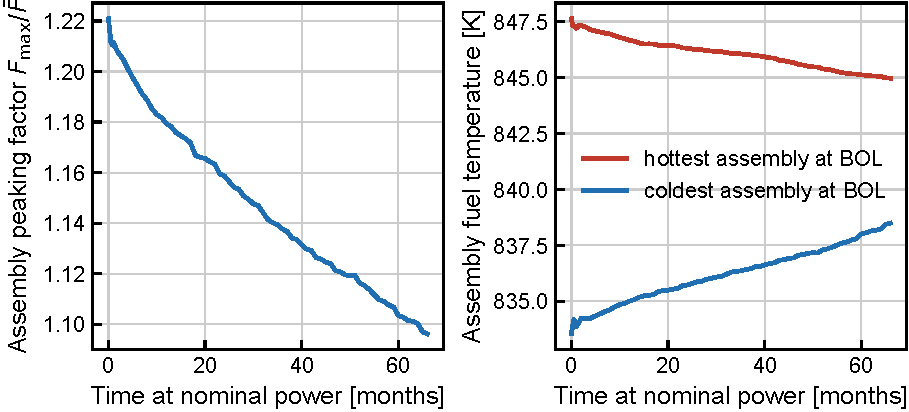
\includegraphics[width=\textwidth]{Chapter7/Figs/power_flattening.pdf}
  \caption[Power flattening over the cycle]{Assembly peaking factor of the
  fission source over the cycle (left) and fuel temperature of the assemblies
  that are hottest and coldest at beginning of life (right).}
  \label{cs:fig:flattening}
\end{figure}

\begin{figure}[htbp]
  \centering
  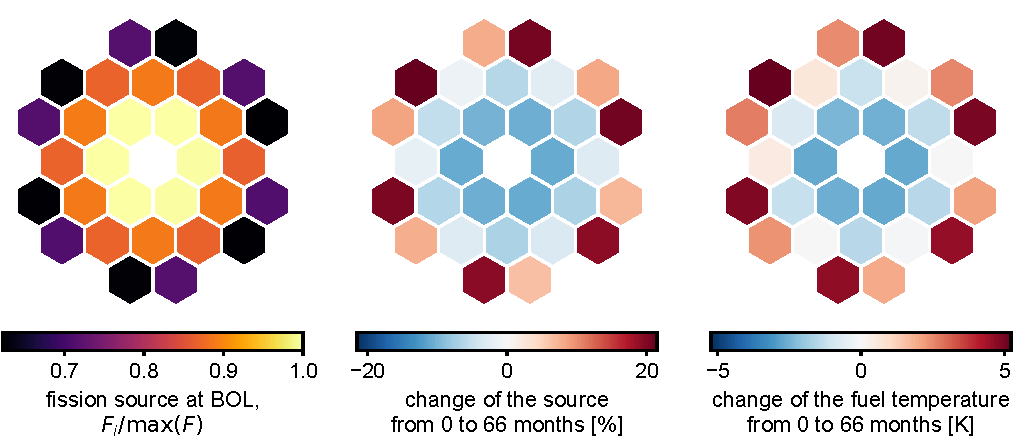
\includegraphics[width=\textwidth]{Chapter7/Figs/bol_eol_maps.pdf}
  \caption[Fission source and temperature redistribution]{Assembly-wise
  normalized fission source at beginning of life (left), its relative change
  between beginning and end of the 66-month window (centre) and the
  corresponding change of the fuel temperature (right).}
  \label{cs:fig:bolmaps}
\end{figure}

The nuclide inventories come directly from the depletion output (see
Figs.~\tref{cs:fig:inventory} and \tref{cs:fig:u235map}). At 66 months the
core-average depletion of $^{235}$U is \SI{5.75}{\percent}, \SI{6.58}{\percent}
in the middle axial zone and \SI{4.28}{\percent} in the top zone, and
\SI{6.59}{\percent} in the most depleted assembly; $^{239}$Pu builds up to
\SI{1.05}{\percent} of the initial
$^{235}$U atoms. The fission share of $^{235}$U decreases from 0.995 to 0.958
and that of $^{239}$Pu reaches \SI{3.6}{\percent}; the conversion ratio
increases from 0.199 to 0.207. The build-up of the two saturating absorbers is
the physical content of the dense early snapshot grid: $^{135}$Xe is at
equilibrium at the first snapshot, $^{149}$Sm reaches it after about two
years. A second depletion, identical in input and with an independent seed,
reproduces the core-total $^{235}$U inventory to \SI{0.013}{\percent}: the
composition noise due to the low-statistics depletion is far below the tally
noise of the snapshot matrices. Hence, the depletion can reasonably be
excluded as a source of error.

\begin{figure}[htbp]
  \centering
  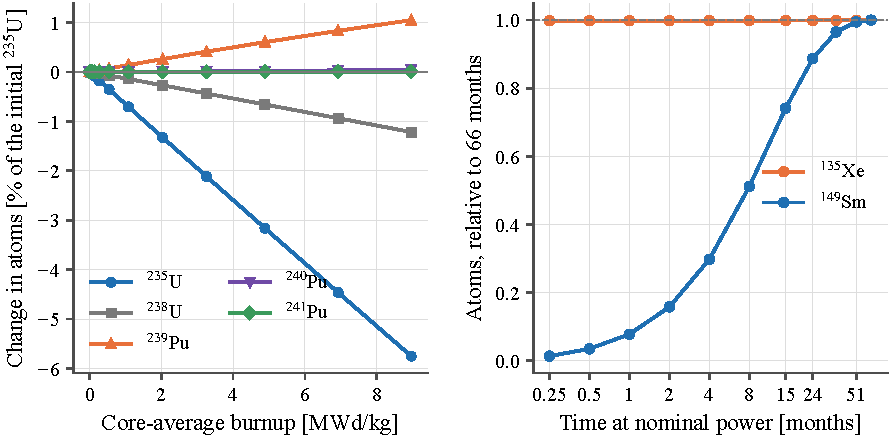
\includegraphics[width=\textwidth]{Chapter7/Figs/inventory.pdf}
  \caption[Fuel inventory over the cycle]{Core-total change of the heavy
  nuclides over the cycle, as a percentage of the initial $^{235}$U atoms (left),
  and build-up of $^{135}$Xe and $^{149}$Sm relative to their value at 66
  months (right), from the depletion output.}
  \label{cs:fig:inventory}
\end{figure}

\begin{figure}[htbp]
  \centering
  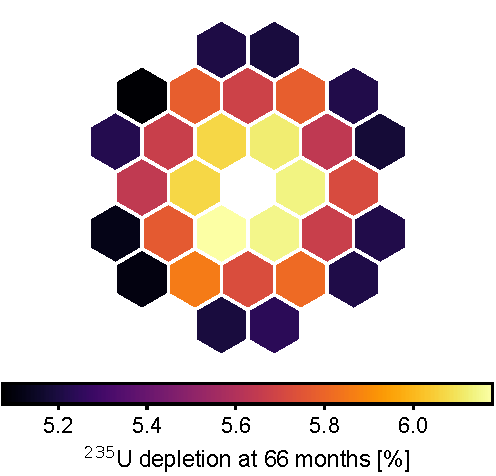
\includegraphics[width=0.47\textwidth]{Chapter7/Figs/u235_depletion_map.pdf}
  \caption[Assembly-wise depletion of uranium-235]{Assembly-wise depletion of
  $^{235}$U at 66 months, from the zone-wise depletion output.}
  \label{cs:fig:u235map}
\end{figure}

\section{Assessment of the three assumptions of the
factorization}\label{cs:sec:hypotheses}

\subsection{Angle independence}

The production snapshots are tallied at a single drum angle. To quantify the error introduced by this choice, the snapshot compositions of
the same restart file are re-tallied at four further angles, \ang{45},
\ang{90}, \ang{135} and \ang{180}, at the cost of 48 transport calculations
and no additional depletion. The test compares tallied matrices
only, with no interpolation. At each angle $\theta'$ and snapshot time $t_s$,
%
\begin{equation}
  \Delta k(\theta', t_s) \;=\;
  k\big[\,a^{\mathrm{tally}}(\theta',0)\cdot \mathrm{BCR}(t_s)\,\big]
  \;-\; k\big[\,a^{\mathrm{tally}}(\theta', t_s)\,\big],
  \label{cs:eq:thetatest}
\end{equation}
%
where the first term is the eigenvalue obtained under the angle-independence
hypothesis, from the fresh matrix tallied at $\theta'$ corrected with the
reference-angle ratio, and the second is that of the matrix tallied directly
at $\theta'$ and $t_s$. Each point carries the
statistics of four independent tallies, the two matrices at $\theta'$ and the
two behind the ratio, about \SI{22}{pcm} on $k_{\mathrm{eff}}$, and that is
the resolution against which the structural error is judged. The 44 measured
points (see Fig.~\tref{cs:fig:theta}) have a root-mean-square of \SI{23}{pcm}
and none of them is beyond \SI{59}{pcm}; the means over the cycle at the four
angles are $-19$, $+11$, $+5$ and $+2$~pcm. Within the \SI{22}{pcm} resolution
of the test, the error $\Delta k(\theta',t_s)$ is therefore independent of both
burnup and drum angle: it shows no systematic variation along the cycle, and
it does not grow as $\theta'$ moves away from the reference angle. The
hypothesis thus holds at every angle, the \ang{180} corner included, which is where a shutdown-margin evaluation would apply the
ratio farthest from its tally point.

\begin{figure}[htbp]
  \centering
  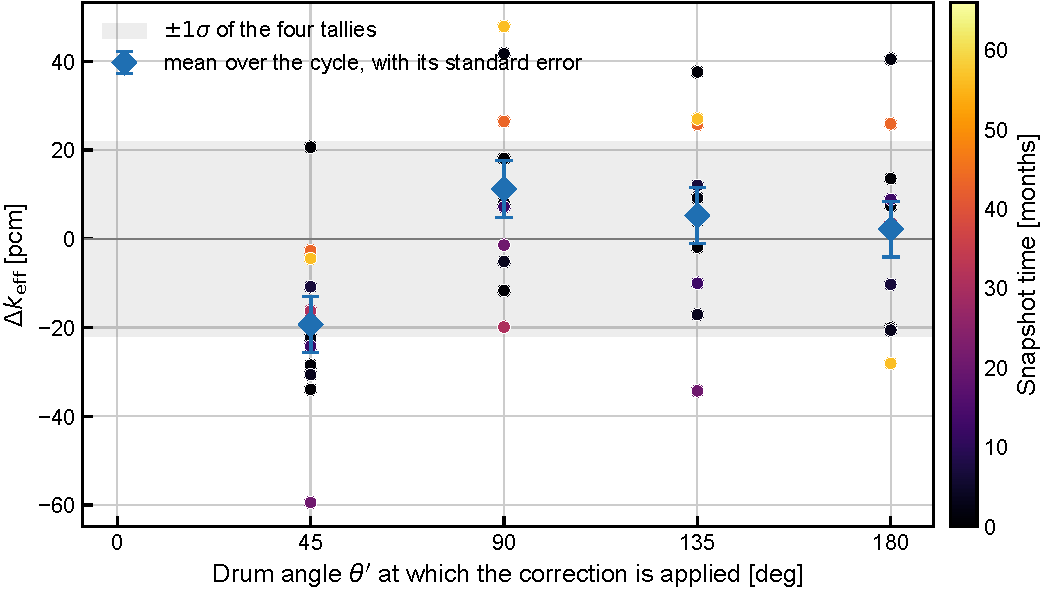
\includegraphics[width=\textwidth]{Chapter7/Figs/theta_independence.pdf}
  \caption[Angle-independence test of the burnup correction]{Structural error
  of the angle-independent Burnup Correction Ratio, Eq.~(\ref{cs:eq:thetatest}),
  at the four drum angles where the snapshot compositions are re-tallied: one
  point per snapshot time (colour), the mean over the cycle with its standard
  error, and the $\pm1\sigma$ band expected from the statistics of the four
  tallies behind each point.}
  \label{cs:fig:theta}
\end{figure}

The effect on the critical drum angle over the cycle is also checked, by
running the cycle with the ratio interpolated between the five tallied angles
instead of being taken from the single reference angle,
$\theta_{\mathrm{ref}}=\ang{0}$ (see Fig.~\tref{cs:fig:thetacost}). The
critical angle differs
from the single-angle cycle by \ang{0.69} on average and \ang{1.54} at most,
at 24 months; through the local drum worth of \SI{55}{pcm} per degree at that
time, the maximum corresponds to \SI{85}{pcm} and the mean to \SI{38}{pcm}.
These differences reflect the tally statistics of the five-angle variant
itself: between two tallied planes the ratio is interpolated from matrices
each of which carries the noise of two independent tallies, so that the
deviation from the single-angle variant is dominated by statistical noise. In
agreement with the absence of structural error found above, this deviation is
therefore not an error introduced by the angle-independence hypothesis.

\begin{figure}[htbp]
  \centering
  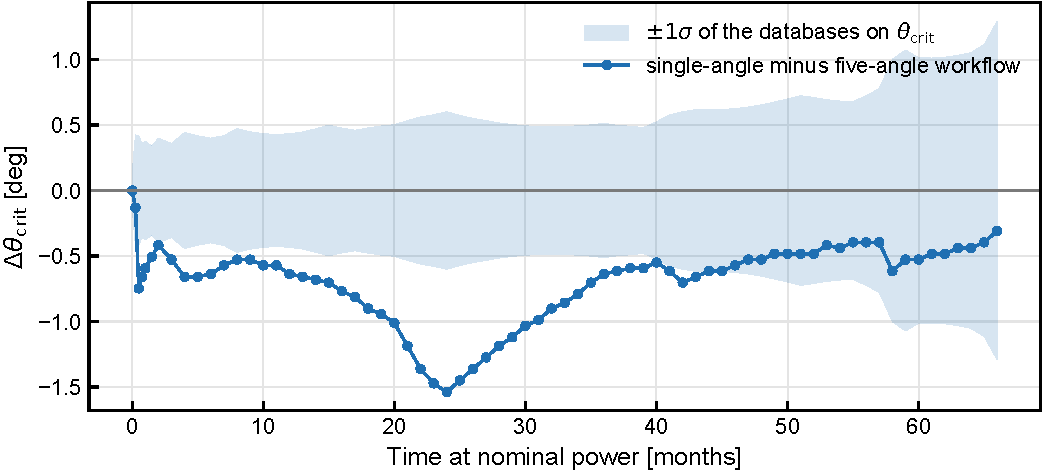
\includegraphics[width=\textwidth]{Chapter7/Figs/theta_cost.pdf}
  \caption[Effect of the angle resolution of the correction on the critical
  angle]{Difference of the critical drum angle over the cycle between the
  single-angle workflow, with the Burnup Correction Ratio tallied at the
  reference angle $\theta_{\mathrm{ref}}=\ang{0}$ only, and the five-angle
  workflow, with the ratio interpolated between the tallied angles \ang{0},
  \ang{45}, \ang{90}, \ang{135} and \ang{180}, against the $\pm1\sigma$ band of
  the databases on the critical angle.}
  \label{cs:fig:thetacost}
\end{figure}

\subsection{Fixed temperature}

The snapshots are tallied at the fixed nominal temperature state, so that the
ratio isolates the composition effect. The temperature dependence is carried
by the interpolation of Eq.~(\ref{cs:eq:interp}), and letting the snapshots
follow the evolving profile would count it twice. The factorization neglects
the cross-term between temperature and burnup, that is, the dependence of the
burnup response itself on the temperature state. This is measured with one
dedicated transport simulation: the 51-month composition is re-tallied in the
evolved temperature state, that is, with the fuel temperature field that the
workflow obtains from the fission source through
Eq.~(\ref{cs:eq:correlation}). As the source flattens over the cycle, this
field departs from the reference temperature state by a redistribution of up
to \SI{+10}{K}. The tally is compared with the reference-state snapshot of the
same composition, at the same drum angle and with an independent seed. The result, $\Delta k_{\mathrm{eff}}=-9\pm15$~pcm, is compatible with zero
within the statistical uncertainty. Figure~\tref{cs:fig:frozen} compares the
two tallies coefficient by coefficient. For the dominant coefficients, the
largest \SI{25}{\percent} of the non-zero coefficients of the fresh-fuel matrix,
the correction ratios have the same median in the two cases, 0.9775 against 0.9776, and their differences are
distributed as the tally noise predicts, with an expected per-coefficient
standard deviation of 0.021.

\begin{figure}[htbp]
  \centering
  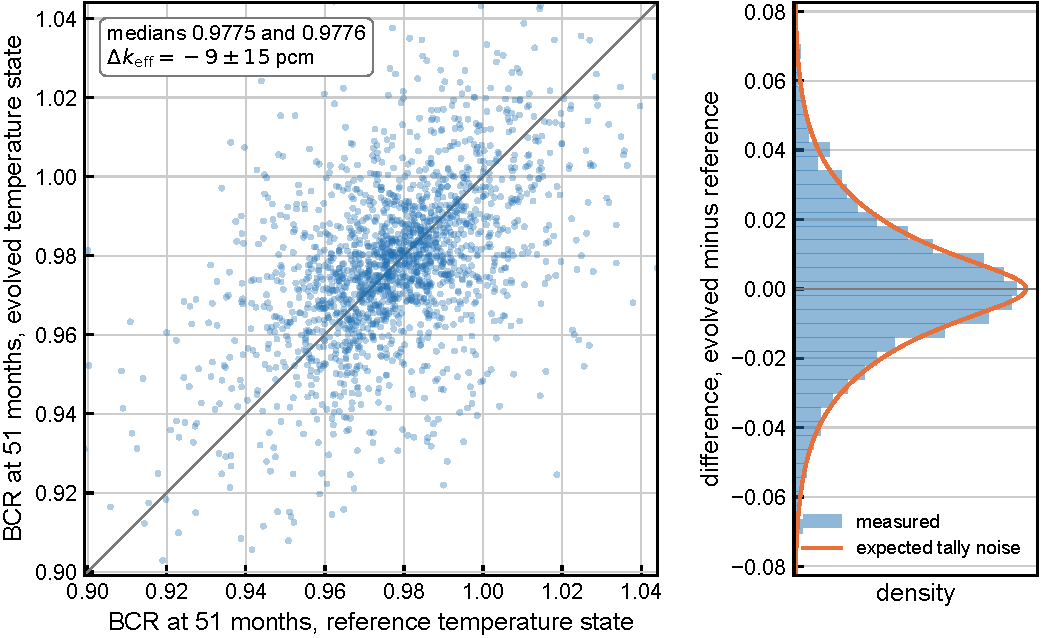
\includegraphics[width=\textwidth]{Chapter7/Figs/frozen_temperature.pdf}
  \caption[Fixed-temperature test of the burnup correction]{Burnup Correction
  Ratio at 51 months for the dominant coefficients (upper quarter of the
  fresh-fuel matrix), tallied in the evolved temperature state computed by the
  workflow against the reference temperature state (left), and distribution of the
  differences compared with the expected tally noise (right).}
  \label{cs:fig:frozen}
\end{figure}

\subsection{Single history}

The production depletion runs with the drums fully extracted, while the
operating reactor keeps them on the critical trajectory. With the drums
inserted, the flux in the drum-adjacent periphery is depressed and the
depletion of those assemblies proceeds more slowly. The hypothesis is measured with a
second depletion, identical to the first except for the drums, frozen at
\ang{33.75}, which is the database angle closest to the time average of the critical
trajectory. Its compositions are re-tallied at the standard conditions at four
snapshot times. Table~\tref{cs:tab:history} and Fig.~\tref{cs:fig:history} give
the effect on the tallied matrices and the effect that survives in the
workflow, where the ratio from the alternative history replaces the production
one on the interpolated matrix. The compositions move $k_{\mathrm{eff}}$ by at
most \SI{27}{pcm}, with a change of sign around mid-cycle, since the shielded
periphery burns more slowly at first and catches up later. The workflow moves
by at most \SI{58}{pcm} at mid-cycle and by \SI{3}{pcm} at end of life: the
cycle length, read at the drums-out crossing, is insensitive to the drum
history assumed in the depletion.

\begin{table}[htbp]
  \centering
  \caption[Single-history test]{Single-history test: change of the
  multiplication factor when the compositions of the depletion with the drums
  frozen at \ang{33.75} replace those of the production depletion, drums
  fully extracted, at four snapshot times. The first row compares the
  matrices tallied from the two sets of compositions at the standard
  conditions; the second compares the workflow at its critical state, with the
  burnup correction ratio of one history replacing that of the other. The
  statistical uncertainty of an entry, from the two and the four independent
  tallies that enter it, is about 16 and \SI{22}{pcm} respectively.}
  \label{cs:tab:history}
  \begin{tabular}{lcccc}
    \toprule
    & \multicolumn{4}{c}{$\Delta k_{\mathrm{eff}}$ (pcm)} \\
    \cmidrule(lr){2-5}
    Snapshot time (months) & 8 & 24 & 51 & 66 \\
    \midrule
    Tallied matrices, $\pm16$~pcm & $+22$ & $+27$ & $-26$ & $-26$ \\
    Workflow, $\pm22$~pcm         & $+54$ & $+58$ & $+4$  & $+3$  \\
    \bottomrule
  \end{tabular}
\end{table}

\begin{figure}[htbp]
  \centering
  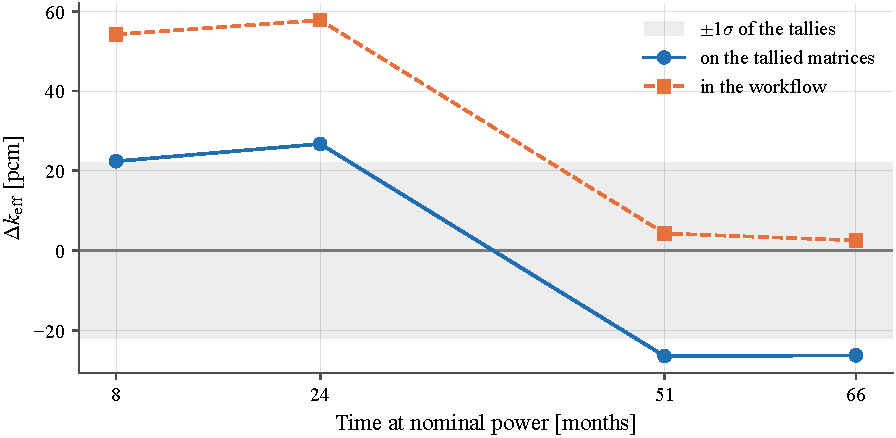
\includegraphics[width=\textwidth]{Chapter7/Figs/single_history.pdf}
  \caption[Single-history test of the burnup correction]{Effect of the drum
  history of the depletion on the multiplication factor, on the tallied
  matrices and in the workflow, against the $\pm1\sigma$ band of the tally
  statistics.}
  \label{cs:fig:history}
\end{figure}

\section{Density of the snapshot grid}\label{cs:sec:grid}

The number of snapshot times required is determined with the acceptance method
of Sec.~\ref{cs:sec:selection}, applied to the burnup axis. Nested sub-grids of
the twelve-point grid, of 2, 4 and 7 points, are tested at the midpoints of
the full grid, where the time-interpolation error peaks. At each test time the
workflow gives the critical state on the full database, and every sub-grid is
evaluated at that frozen state, so that $\Delta k_{\mathrm{eff}}$ isolates the
effect of the density. The full grid reproduces the states it defines to
\SI{0.4}{pcm}, i.e., the search tolerance, which is the floor of the test.
Against it (see Fig.~\tref{cs:fig:grid} and Table~\tref{cs:tab:grid}), the
interpolation error falls from \SI{297}{pcm} with two snapshot times to \SI{80}{pcm} with
four and to \SI{21}{pcm} with seven, where it first enters the \SI{22}{pcm}
band of the reference statistics. Seven snapshot times are therefore
sufficient on the burnup axis of this design. Beyond that number, the residual is dominated by the tally noise that the
ratio carries as a quotient of two independent runs, and it could be reduced
only by increasing the number of histories per snapshot, not the number of
snapshot times.

\begin{figure}[htbp]
  \centering
  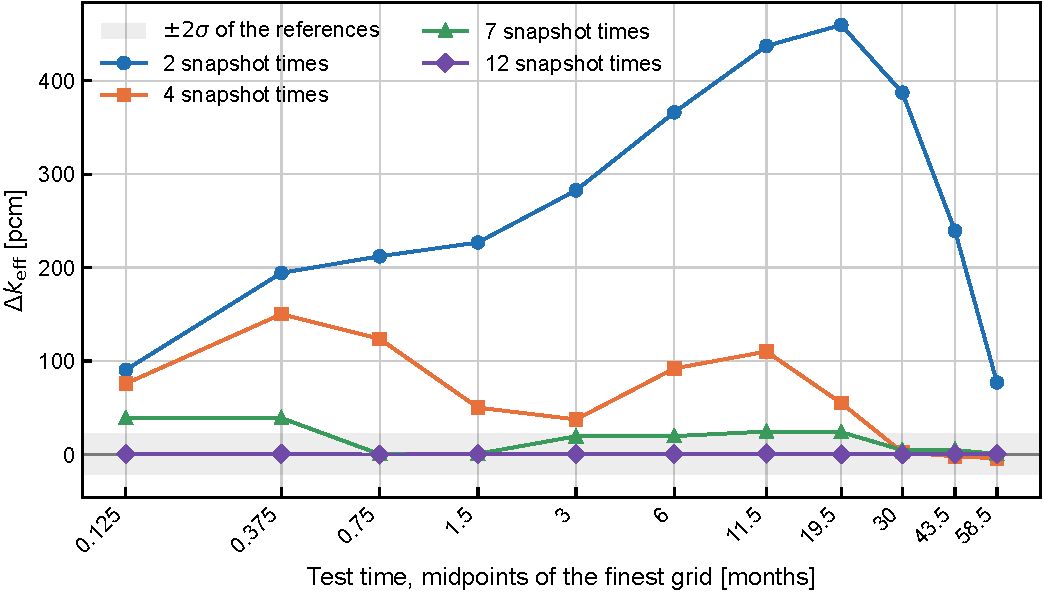
\includegraphics[width=\textwidth]{Chapter7/Figs/snapshot_grid_density.pdf}
  \caption[Interpolation error against snapshot-grid density]{Time-interpolation
  error of nested snapshot grids of 2, 4, 7 and 12 points, evaluated at the
  midpoints of the full grid at the critical state given by the workflow,
  compared with the $\pm2\sigma$ statistics of the reference calculations.}
  \label{cs:fig:grid}
\end{figure}

\begin{table}[htbp]
  \centering
  \caption[Interpolation error against snapshot-grid density]{Interpolation
  error of the nested snapshot grids at the eleven midpoints of the full grid:
  smallest, largest and root-mean-square deviation of the multiplication
  factor (pcm). The statistical uncertainty of the references is
  \SI{11}{pcm}.}
  \label{cs:tab:grid}
  \begin{tabular}{lS[table-format=-2.1]S[table-format=3.1]S[table-format=3.1]}
    \toprule
    Snapshot grid & {min $\Delta k_{\mathrm{eff}}$} & {max $\Delta k_{\mathrm{eff}}$} & {RMSE} \\
    \midrule
     2 points &  76.9 & 459.7 & 297.3 \\
     4 points &  -4.2 & 150.1 &  80.4 \\
     7 points &   0.1 &  38.9 &  21.2 \\
    12 points &  -0.3 &   0.8 &   0.4 \\
    \bottomrule
  \end{tabular}
\end{table}

\section{Computational cost}\label{cs:sec:cost}

Table~\tref{cs:tab:cost} gathers the data related to the Serpent~2 campaigns
needed to support the workflow, that is, the cost paid once before any search is run, together with the
cost of the workflow itself. The database of Sec.~\ref{cs:sec:database} is
generated on a thirty-core workstation with an Intel Xeon Gold 6130 processor
at \SI{2.1}{GHz}: 136 criticality calculations, about \SI{63}{CPU\,h} each,
\SI{324}{h} of wall-clock time in all. The burnup extension adds one depletion
calculation and the twelve snapshot transports restarted from it. The upfront
cost amounts to about \SI{9500}{CPU\,h}, nine tenths of which are the
$(T,\theta)$ database. Against it, the workflow runs on a single core of a
personal computer: a search that neglects the Monte Carlo uncertainty of the
database takes tens of milliseconds, a search
with the uncertainty ensemble about one second, and the complete 66-month
cycle, 71 steps with fifty realizations at each step, \SI{40}{s}.

The campaigns run to verify the workflow and to measure its assumptions are
listed separately in Table~\tref{cs:tab:testcost}, because they are not part
of the cost of the method: an application would not repeat them. They amount to
66 transports and one further depletion, about \SI{4500}{CPU\,h}, all
restarted from the production depletion except the history test, which has a
depletion of its own.

\begin{table}[htbp]
  \centering
  \caption[Upfront campaigns and cost of the workflow]{Serpent~2 campaigns
  paid once, before any search (transports at $10^{5}$ neutrons per cycle and
  500 active cycles), and cost of the fission matrix workflow, measured on one
  core.}
  \label{cs:tab:cost}
  \begin{tabular}{p{74mm}cc}
    \toprule
    Campaign & Runs & Cost \\
    \midrule
    $(T,\theta)$ database, Sec.~\ref{cs:sec:database} & 136 & \SI{63}{CPU\,h} each \\
    Depletion at the reference state, drums fully extracted & 1 & \SI{2.75}{h} on 64 cores \\
    Snapshot matrices at $\theta_{\mathrm{ref}}=\ang{0}$, Sec.~\ref{cs:sec:snapshots} & 12 & \SI{66}{CPU\,h} each \\
    \midrule
    Search, Monte Carlo uncertainty neglected & -- & \SI{29}{ms} \\
    Search, ensemble of 100 realizations included & -- & \SI{1.1}{s} \\
    Cycle, 71 steps, ensemble of 50 realizations & -- & \SI{40}{s} \\
    \bottomrule
  \end{tabular}
\end{table}

\begin{table}[htbp]
  \centering
  \caption[Verification and assumption-test campaigns]{Serpent~2 campaigns
  run to verify the workflow and to measure the assumptions of the burnup
  correction, Sec.~\ref{cs:sec:hypotheses}; same statistics as the database
  entries.}
  \label{cs:tab:testcost}
  \begin{tabular}{p{74mm}cc}
    \toprule
    Campaign & Runs & Cost \\
    \midrule
    Reference criticality calculations along the cycle & 12 & \SI{62}{CPU\,h} each \\
    Snapshots re-tallied at \ang{45}, \ang{90}, \ang{135} and \ang{180} (angle independence) & 48 & \SI{66}{CPU\,h} each \\
    Snapshot re-tallied at the evolved temperature (fixed temperature) & 1 & \SI{66}{CPU\,h} \\
    Depletion with the drums frozen at \ang{33.75} (single history) & 1 & \SI{2.75}{h} on 64 cores \\
    Snapshots of that history, re-tallied at the standard conditions & 5 & \SI{66}{CPU\,h} each \\
    \bottomrule
  \end{tabular}
\end{table}

\section{Summary}

The criticality search of this chapter rests on a database of 136 fission
matrices over eight temperatures and seventeen drum angles, whose density is
settled by a nested convergence study, and on a prescribed correlation between
power and fuel temperature that makes the search self-consistent.
At nominal power and fresh fuel the search converges in about one second on a
single core, uncertainty quantification included, and the multiplication
factor at the state it returns deviates from a reference Monte Carlo
calculation by $-56\pm16$~pcm, the interpolation residual of the database.

The extension to burnup adds no dimension to the database. Burnup enters the
interpolated matrix as a multiplicative correction ratio, tallied once per
snapshot time at a single reference angle and temperature state; one
low-statistics depletion gives the compositions, and twelve independent
transports restarted from it tally the snapshot matrices. The workflow then
drives a quasi-static cycle in which drum position, temperature field, fission
source and cell-wise burnup are updated together at every step. Reference
calculations at the states returned by the algorithm put $k_{\mathrm{eff}}$
within $-59$ to $-5$~pcm of unity over 66 months, with the bias already
present at beginning of life and no drift with burnup; the assembly-wise
fission source agrees to about \SI{1}{\percent}. The three assumptions of the
factorization are measured on dedicated campaigns and found at or below that
residual: the angle independence holds at the \SI{22}{pcm} resolution of the
test at every angle up to \ang{180}, the temperature--burnup cross-term is
$-9\pm15$~pcm, and the drum history behind the compositions moves the
workflow by at most \SI{58}{pcm} at mid-cycle and by \SI{3}{pcm} at end of
life. Seven snapshot times suffice on the burnup axis.

The residual of the method is the interpolation of the original database, not
the burnup correction. Two developments follow from it. The first is the
treatment of the effects that the isothermal database cannot represent, the
temperature difference between core and reflector first of all, which is the
subject of Chapter~\ref{ch:correction-ratios}. The second is the replacement
of the correlation of Eq.~(\ref{cs:eq:correlation}) with a thermal response
from a conduction solver, which the interface of the workflow already allows.
